\documentclass[letterpaper,journal,onecolumn]{IEEEtran}
\usepackage[T1]{fontenc}
\usepackage[utf8]{inputenc}
\usepackage{amsmath,amssymb,graphicx,booktabs,array,tabularx,ragged2e,textcomp,url,xurl,cite,stfloats,placeins}
\usepackage[hidelinks]{hyperref}
\graphicspath{{../figs/}}
\urlstyle{same}
\providecommand{\tightlist}{\setlength{\itemsep}{0pt}\setlength{\parskip}{0pt}}
\setlength{\emergencystretch}{1.5em}
\hyphenation{rein-force-ment en-vi-ron-ment accel-er-a-tion}
\pagestyle{plain}

\begin{document}
\title{Supplementary Material\\Environment-Aware Reinforcement Learning for Electric Vehicle Eco-Driving with Smooth Execution}\author{Ziran Peng and Zeyu Fan}\maketitle
Sections A--C support the system and interfaces in main Section III; D supports execution in Section IV; E supports the preparation reference in Section V. Sections F--I follow the evaluation order in main Section VI: comfort and timing, visual driving, preparation and target diagnosis, then the structured 20 km reference. Section J specifies reproduction and data availability. References use the same citation keys as the main manuscript.

\FloatBarrier\stepcounter{section}\section*{A. VEHICLE MODEL AND STRUCTURED OBSERVATIONS}\setcounter{subsection}{0}

\subsection*{A.1. Traction and regenerative power}

The longitudinal parameters follow the 2019 Nissan Leaf Plus benchmarking report \cite{S4}: test mass \(m=1928\) kg and coast-down road load

\[F_{\rm road}(v)=A+Bv+Cv^2,\qquad A\approx135.05\ {\rm N},\quad B\approx3.1851\ {\rm N\,s/m},\quad C\approx0.43626\ {\rm N\,s^2/m^2}. \tag{A1}\]

The displayed road-load coefficients are rounded; computation retains the original coast-down unit conversions. Rolling radius is 0.3234 m, final-drive ratio 8.139, and motor ratings are 340 N·m and 160 kW, corresponding to \(F_{\max}=340(8.139)/0.3234\approx8556.77\) N and base speed 18.7 m/s. The road is flat. The battery is parameterized separately below. For achieved acceleration \(a\),

\[F_w=ma+F_{\rm road}(v),\qquad P_w=F_wv. \tag{A2}\]

\textbf{Implemented efficiency model.} The loss function used to construct the efficiency map is

\[P_{\rm loss}(F,v)=P_0+k_{\rm Fe}v+k_{\rm Cu}F^2. \tag{A3}\]

Here \(P_0=300\) W is an assumed standby term; \(k_{\rm Fe}\approx32.4\) W·s/m and \(k_{\rm Cu}\approx1.07\times10^{-4}\) W/N\textsuperscript{2} are solved from two specified operating anchors: 96\% at 4000 N and 15 m/s, and 90\% at 421 N and 22.22 m/s. The 96\% level follows \cite{S4}; the selected operating coordinates, standby term, and cruise anchor define the engineering calibration.

For the implemented map, let \(v_\epsilon=\max(v,10^{-3})\), \(F_{\rm mot}(v)=\min(F_{\max},160000/v_\epsilon)\), and \(\bar F=\min(\max(F,0),F_{\rm mot}(v))\). Both power-flow branches use

\[\eta_c(F,v)=\operatorname{clip}\!\left[
\frac{\bar Fv_\epsilon}{\bar Fv_\epsilon+P_{\rm loss}(\bar F,v_\epsilon)},\,0.05,\,0.97
\right].\]

Traction evaluates \(\eta_c\) at \(F_w\), and regeneration evaluates it at the actual regenerative force. Using the same map for regeneration is an engineering approximation; the implemented regeneration branch does not use \((P_{\rm mech}-P_{\rm loss})/P_{\rm mech}\). The reduction-gear efficiency is \(\eta_{\rm tr}=0.97\) and the high-voltage auxiliary load is \(P_{\rm aux}=167/0.86\approx194\) W \cite{S4}. At steady 80 km/h the model consumes approximately 136 Wh/km.

\subsection*{A.2. Battery and charge acceptance}

The parameterized pack has 96 series groups and two parallel 50 Ah NMC cells per group. A nominal cell voltage of 3.65 V sets its stored energy to 35040 Wh. For clipped SOC \(s\in[0,1]\), the implemented empirical open-circuit voltage is \(U_{\rm oc}(s)=3.20+0.90s^{0.55}+0.12s^6\) V. Its endpoint is 4.22 V; the charge-headroom voltage limit is separately set to \(U_{\max}=4.20\) V.

The per-cell resistance is \(R_0(T)=1.5\times10^{-3}\exp[2100(1/T-1/298.15)]\) ohm. With \([z]_+=\max(z,0)\), the pulse charge-acceptance ceiling is

\[P_{\rm acc}(s,T)=
\min\!\left\{
n_sn_pU_{\rm oc}(s)
\left[\frac{U_{\max}-U_{\rm oc}(s)}{R_0(T)}\right]_+,\,
P_{\rm hw}
\right\},\qquad P_{\rm hw}=90\ {\rm kW}. \tag{A4}\]

The positive part sets acceptance to zero where the empirical OCV exceeds the voltage limit. Nominal stored energy, the OCV curve, and the pulse ceiling are engineering model components informed by \cite{S3}, \cite{S5}; they do not constitute a complete chemistry, aging, or charging-safety model. Temperature is fixed within a trip.

\textbf{Braking split.} For \(v\ge2\) m/s and \(P_w<0\), the implemented mechanical ceiling is the fixed point

\[F_{\rm ceil}
=\min\!\left\{F_{\rm mot}(v),
\frac{P_{\rm acc}+P_{\rm aux}}{v\,\eta_c(F_{\rm ceil},v)}\right\},
\quad F_{\rm reg}=\min(-F_w,F_{\rm ceil}),
\quad F_{\rm fric}=-F_w-F_{\rm reg}. \tag{A5}\]

The code uses a damped fixed-point iteration capped at 40 iterations. For \(v<2\) m/s, regenerative braking is disabled and braking uses friction; low-speed traction remains available. Battery power is

\[P_b=\begin{cases}
P_w/[\eta_{\rm tr}\eta_c(F_w,v)]+P_{\rm aux},&P_w\ge0,\\
-F_{\rm reg}v\,\eta_{\rm tr}\eta_c(F_{\rm reg},v)+P_{\rm aux},&P_w<0,\ v\ge2,\\
P_{\rm aux},&P_w<0,\ v<2,
\end{cases}
\qquad \dot s=-P_b/E_{\rm pack}. \tag{A6}\]

The ceiling is applied before gear loss, so the net power received by the pack is at most \(\eta_{\rm tr}P_{\rm acc}\), up to iteration tolerance. The ledger is \(E_b=\int P_b\,dt\), \(E_{\rm fric}=\int F_{\rm fric}v\,dt\), and \(E_{\rm reg}=\int\max(-P_b,0)\,dt\). Equation (A6) gives \(E_b=-\Delta s\,E_{\rm pack}\); derived SOC entries are accounting conversions rather than independent logged measurements. All controllers share this model.

\subsection*{A.3. Structured-input normalization}

The following thirteen-channel observation belongs to the structured-input configurations and the 20 km reference study. P-V uses camera-derived memory and the expanded input in Section B; simulator road truth is not a runtime visual-policy input.

The policy receives thirteen channels. The simulator also contains signal offsets that are not fully observed outside broadcast range. Thus this is a policy observation, not a claim of complete state observability.

\[o = \Big[\tfrac{v}{v_{\max}},\ \tfrac{a}{3.5},\ \tfrac{d_{\text{end}}}{L},\ \tfrac{v_{\lim}(x)}{v_{\max}},\ \tfrac{d_c}{400},\ \tfrac{v_c}{v_{\max}},\ \tfrac{d_s}{1000},\ \phi_s,\ \tau_s,\ \tfrac{\text{SOC}-0.5}{0.5},\ \tfrac{T-283.15}{30},\ \tfrac{t_{\text{end}} - t}{T_b},\ \tfrac{t}{T_b}\Big], \tag{A7}\]

The first nine entries describe speed, previous acceleration, remaining distance, current limit, curve preview within 400 m, and signal distance/phase/time-to-change within 1000 m. Outside signal range the phase/timing code is \((-1,1)\). The final four entries encode SOC, temperature, remaining time to the episode deadline, and elapsed time. Exposing both clocks removes a hidden deadline variable but does not eliminate partial observability of distant signals.

\FloatBarrier\stepcounter{section}\section*{B. VISUAL PERCEPTION, MEMORY, AND LEARNING INTERFACE}\setcounter{subsection}{0}

\subsection*{B.1. Information flow and training protocol}

The main question is whether visual events support completion, traffic compliance, reasonable progress, and smooth execution. Superiority of one encoder-update method is a secondary question. The conditions were used during development, so the analysis is retrospective. No same-condition human-driver or passenger-comfort experiment is available. The driver policies in Section I.2 are programmed references, not measured human driving.

Images are 96 by 160 pixels, sampled every 0.5 s, with a four-frame history. A frozen detector estimates boxes, distance, and signal color; predicted ROI and event memory connect these outputs to the executor. A separate policy encoder supplies Z. F freezes it; S uses visual supervision; J also receives critic feedback along the Z-producing backbone/fusion path; JH opens temporal and signal\_z parameters, with critic feedback only through temporal. All actor updates stop at the encoder. Backward checks of the saved core and weights confirm these routes; the deployed detector remains frozen throughout.

The modes share actor/critic learning rates 3e-5/3e-4, encoder learning rate 1e-5, batch size 32, visual batch size eight sequences, target noise 0.2 clipped at 0.5, Polyak rate 0.005, actor delay two, and replay capacity 6000 decisions. Targets span at most twenty decisions with gamma=1. The 2400-substep common prefix precedes about 9000 arm-specific substeps. All modes use lambda\_c=0.1, so this visual study does not independently isolate the regularizer's effect.

\subsection*{B.2. Event semantics and retained memory}

A warning-sign detection initializes curve-entry distance as estimated sign distance plus 400 m; speed integration updates that distance and a fixed 35 km/h limit applies at estimated entry. A detected exit sign releases the restriction; travel beyond 1000 m after estimated entry is a fallback. Lamp distance is translated to stop-line distance with a fixed 14 m mounting offset. The experiment tests known sign semantics and geometry, not OCR or arbitrary sign values. The 200 m signal rendering range is distinct from reliable detection distance.

The memory uses a 15 m endpoint-distance bias, a 6 m absolute plus 15\% relative approach margin, a stopping latch, and a 10 s stationary no-detection expiration. These rules were developed using seed-0 conditions. A green observation is assigned an assumed 30 s remaining duration. Near-line color commitment can retain an earlier green despite a red measurement; detection loss can clear a light target while stopped. These are memory decisions, not necessarily camera classification failures.

All twelve checkpoints use the original 87-dimensional policy input, including six extra memory features. The optional extra\_dim=10 interface is not used by these weights. It exposes additional latch/commitment/observation fields but does not by itself establish a Markov representation: voting, consistency and release history can still affect future memory transitions. The evaluated logs do not contain its additional observed/observed\_conf/committed fields. Its availability does not change the input used for the reported experiments.

\subsection*{B.3. Visual-supervision objective}

The delivered \path{perception_loss} uses six terms, with the outer learning coefficient \(\lambda_v=1\) in the archived configurations:

\[\mathcal L_{\rm vis}=\mathcal L_{\rm heat}+\mathcal L_{\rm box}
+2\mathcal L_{\rm range}+\mathcal L_{\rm presence}
+\mathcal L_{\rm ROI}+\mathcal L_Z.\tag{B1}\]

Every term is a sum over its valid batch entries divided by the specified valid count, clamped below by one. With binary heat target \(y\), predicted probability \(p\), valid mask \(M\), and \(p_t=py+(1-p)(1-y)\),

\[\begin{aligned}
\mathcal L_{\rm heat}&=\frac{\sum M[0.25y+0.75(1-y)](1-p_t)^2\operatorname{BCE}(p,y)}{\max(1,\sum My)},\\
\mathcal L_{\rm range}&=\frac{\sum M_d\,\operatorname{SL1}_{0.1}\big(\log(1+400\widehat d)-\log(1+400d)\big)}{\max(1,\sum M_d)}.
\end{aligned}\tag{B2}\]

The heat denominator counts positive target cells rather than all image cells. The box term is smooth L1 with transition 1 on valid target cells, divided by the mask expanded over all box components. Distances in (B2) are the normalized network outputs and labels; 400 converts them to metres before the logarithm. \(M\), \(M_d\), and the box mask each include frame validity and the corresponding label-valid mask.

Presence uses binary cross-entropy over valid frames and four event classes. For each class, its positive weight is the batch negative/positive count ratio, with the positive count clamped below by one and the resulting ratio clipped to \([1,20]\). The loss divides by the count of all valid class/frame entries. The ROI term is five-class cross-entropy over valid frames with nonempty ROI; invalid or empty-ROI labels use the ignored index. The \(Z\) term is five-class cross-entropy for the latest valid frame, including unknown, and does not apply the ROI-empty mask. Consequently visual supervision reaches the temporal \(Z\) projection even when the separate ROI head does not contribute. Absent labels contribute zero. Equation (B1) specifies supervision; it does not add actor or critic gradients to the S encoder.

\subsection*{B.4. Implemented actor and critic objectives}

The structured-input short-route objective in main (5) and the visual implementation use different critic-query actions. For the visual actor, let \(y_\theta\) contain its encoded input and let \(\operatorname{sg}\) stop gradients. With normalized feasible first-step bounds \(u_\ell,u_h\),

\[\begin{aligned}
\bar y&=\operatorname{sg}(y_\theta),\qquad u=\pi_\phi(\bar y),\\
u_{\rm STE}&=u+\operatorname{sg}\!\left(\operatorname{clip}_{[u_\ell,u_h]}(u)-u\right).
\end{aligned}\tag{B3}\]

Thus the forward query is clipped while its backward derivative with respect to \(u\) is one. The implemented visual actor objective is

\[\mathcal L_{\rm actor}^{\rm vis}=-\mathbb E\widehat Q_1(\bar y,u_{\rm STE})+\lambda_c\mathbb E\left[(a_{\rm cmd}(u)-a^-)^2\right].\tag{B4}\]

Acceleration is expressed numerically in m/s\(^2\), corresponding to \(a_{\rm ref}=1\) m/s\(^2\) in main (5). The previous actual acceleration is decoded as \(a^-=3.5\,o_{\rm legacy,2}\). Critic parameters are fixed during this actor step, while the derivative through the action argument remains active. Neither term updates the visual encoder.

For the archived visual modes, the critic regression and target are

\[\begin{aligned}
\mathcal L_Q&=\mathbb E\sum_{i=1}^2\left[\widehat Q_i(y_Q,\alpha_t)-b_t\right]^2,\\
b_t&=R_t^{(n)}+d_t^{(n)}\min_{i=1,2}\widehat Q_i^{-}(y_{t+n}^{-},u_{t+n}^{-}),\\
u_{t+n}^{-}&=\operatorname{clip}_{[-1,1]}(\pi^{-}(y_{t+n}^{-})+\epsilon).
\end{aligned}\tag{B5}\]

Here \(\alpha_t\) is the normalized first-substep applied-acceleration label, \(R_t^{(n)}\) the stored multistep return, and \(d_t^{(n)}\) its bootstrap factor, zero on terminal samples. The target command receives clipped TD3 noise but no executor projection. The target networks and \(b_t\) are held constant under differentiation. For F/S, \(y_Q=\operatorname{sg}(y_\theta)\); for J/JH, the permitted encoder parameters remain connected. With the delivered supervised loss \(\mathcal L_{\rm vis}\), the encoder-gradient routes are

\[\nabla_\theta\mathcal L=\begin{cases}
0,&\mathrm{F},\\
\lambda_v\nabla_\theta\mathcal L_{\rm vis},&\mathrm{S},\\
\nabla_\theta\mathcal L_Q+\lambda_v\nabla_\theta\mathcal L_{\rm vis},&\mathrm{J/JH},
\end{cases}\tag{B6}\]

where the last case is restricted to each mode's trainable tensors. The frozen execution detector is separate from \(\theta\). Equations (B3)--(B6) document the actual learner; they do not identify \(\alpha_t\), \(u_{\rm STE}\), and \(u^-_{t+n}\) as equivalent actions or assert a corrected Bellman model.

The learner uses first-substep applied acceleration as the critic action label for a held 2 s command, but queries target critics with an unprojected target-actor command. Actor updates use a straight-through first-step interval clip. The released implementation contains no compensation that makes those three action meanings identical. This is an implementation limitation, not proof of its contribution to every seed difference.

A controlled executor probe demonstrates the label ambiguity. Starting at x=0, v=10 m/s, a=0 with empty visual memory, held commands 1 and 2 m/s\^{}2 yield four-substep acceleration sequences {[}1,1,1,1{]} and {[}1,2,2,2{]}. Their first normalized applied label is identical, 0.384615, but final speeds are 12.0 and 13.5 m/s and 2 s returns are -0.675580 and -1.080769. This probe tests the action interface, rather than learned-policy performance.

Thus the first applied acceleration is insufficient to identify the held-command transition in these records. The F/S comparison evaluates policies produced by this implementation; the J/JH results cannot isolate an advantage of critic-driven representation learning.

\FloatBarrier\stepcounter{section}\section*{C. REUSABLE ENVIRONMENT INTERFACE}\setcounter{subsection}{0}

\subsection*{C.1. Installation, contracts, and verification}

EvcRL 0.1.0 packages the supplied longitudinal plant, procedural camera, camera-event memory, and release-aware executor behind Gymnasium reset/step interfaces. Source provenance records original module hashes; relative imports and per-instance route/execution configuration replace experiment-wide import mutations. Source and a wheel support local installation. The companion is not published to PyPI, and packaging is not a vehicle-performance experiment.

Camera mode uses the 4 km visual protocol's observation dimensions and event-rendering conventions; structured mode exposes the archived 20 km road-input setting separately. Default camera observations contain RGB and six ego quantities. The optional detector callback receives only RGB and returns detections and phase probabilities; the environment does not deliver truth event labels or ROI to this callback. A default installation attaches no trained detector or S policy and therefore does not claim the visual study's task completion rate. Existing weights remain in their separately identified archive.

The public action is a raw normalized command held for up to four physical substeps. Transitions record the public command and actual substep accelerations distinctly. A future learner should train its command-value critic on this public action, not substitute the first applied acceleration as though it represented the whole transition. The archived visual critic's inconsistent labels are not adopted as a recommended learner. An observation containing images and selected memory is still partially observed.

The reproduction profile retains the original memory rules and 600/1312.5 s intrinsic deadlines by route. Optional removal of that deadline changes the task and cannot relabel historical results. An independent external episode cap produces truncation rather than an intrinsic terminal outcome. Local snapshots preserve the full environment state, camera randomness, and pending observation history at public-step boundaries; external stateful detector adapters must supply their state hooks. These are environment snapshots, not a substitute for replay buffers, optimizers, target networks, and RNG states in full training recovery.

Ten software tests check registered Gymnasium interfaces, deterministic seeded behavior, snapshot recovery, simultaneous instance isolation, command holding, reward/energy accumulation, terminal versus truncated outcomes, supported sampled release bounds, and the candidate memory update. The finite API and smoke steps are software verification, distinct from the paper's frozen-policy driving experiments. CPU installation and command-line smoke checks require no Torch or CUDA import. SOFTWARE\_VERIFICATION.json records tested distributions and commands. The companion provides a concrete reuse interface while leaving trained-policy quality, broader scenarios, calibrated error bounds, and real-road transfer unclaimed.

\FloatBarrier\stepcounter{section}\section*{D. RELEASE-AWARE EXECUTION AND TARGET REVISION}\setcounter{subsection}{0}

\subsection*{D.1. Release inverse, backup recursion, and retained intervals}

For current \(a^-=-b\le0\), the fastest admissible release toward zero executes subsequent braking magnitudes \((b-iq)_+\), \(i=1,2,\ldots\), with \(q=j_{\max}\Delta t\). Any other jerk-admissible release retains at least these braking magnitudes until reaching zero acceleration, and therefore loses at least \(W_{\Delta t}(b)\) speed. If \(v\ge W_{\Delta t}(b)\), executing this release leaves every intermediate speed nonnegative because its partial losses are bounded by the total. This proves necessity and sufficiency for the velocity-only release problem. Including a candidate braking step adds the \(i=0\) term. Stopping position and future road constraints must be checked separately by the backups in main Section IV-C.

The release and target checks have a hierarchical relationship. In the delivered base executor, backup\_distance first rejects a negative release reserve. Therefore a finite-distance stopping backup with nonnegative target margin already passes the release screen, subject to code tolerances. The release formula explains the velocity prerequisite; the backup-distance test adds the target geometry and subsequent brake/release trajectory. These are not statistically independent treatments. Main (10) evaluates the next candidate state, and the complete-layer results do not identify separate causal contributions of either check.

The release inverse used by the code can be evaluated without numerical optimization. Write \(q=j_{\max}\delta\) and choose the first integer \(n\) for which

\[b_n=\frac{v/\delta+q n(n-1)/2}{n}\le nq,
\qquad \bar b(v)=\min\{b_n,3.5\}.\tag{D1}\]

The tested limits \(j_{\max}=2,3,4\) and \(\delta=0.5\) require at most four terms, including the proposed braking step. Negative input reserves are clipped to zero. This is the inverse of the piecewise-linear speed-loss sum in main (8), not a new trajectory optimizer.

\textbf{Specified backup recursion.} Initialize \(d=0\) at the supplied \((v,a)\) and reject \(v-W_\delta((-a)_+)<-10^{-8}\). For at most 100 steps, accept a stopping terminal state when \(v\le10^{-9}\) and \(|a|<10^{-9}\); for \(v_T>0\), accept \(v\le v_T+10^{-9}\) with \(a\le0\). Otherwise choose

\[\beta=\begin{cases}
\min(0,a+q),&v\le v_T+10^{-9},\ a<0,\\
\max(0,a-q),&v\le v_T+10^{-9},\ a\ge0,\\
\max\{-3.5,a-q,-\bar b(v-v_T)\},&v>v_T+10^{-9}.
\end{cases}\tag{D2}\]

In the last case, if \(\beta>a+q+10^{-8}\), replace \(\bar b(v-v_T)\) by \(\bar b(v)\): a positive target speed may be undershot while releasing, but physical speed may not become negative. Reject \(\beta>a+q+10^{-7}\) or \(v+\delta\beta<-10^{-8}\). Each accepted step updates

\[v^+=\max(v+\delta\beta,0),\qquad
d^+=d+\tfrac\delta2(v+v^+),\qquad a^+=\beta.\tag{D3}\]

Exhausting the step budget returns infinity. A positive speed target is a cap rather than a requirement to settle at exactly that speed. The interval check also accepts a state already below the cap when the remaining positive-acceleration release cannot cross it: \(v^++\delta\sum_{i\ge1}(\beta-iq)_+\le v_T+10^{-9}\).

\textbf{Candidate search and wrappers.} The base lower bound is \(\max\{-3.5,a-q,-\bar b(v)\}\) and its upper bound is \(\min\{2.6,a+q,\bar b((v_{\max}-v)_+)\}\) when a speed cap is supplied. A lower bound above the upper by more than \(10^{-9}\) is infeasible. For each target, failure of the lower candidate's next-step distance check with \(10^{-7}\) m tolerance returns \path{stop_distance_infeasible}. A tolerance-only pass retains just the lower endpoint. Otherwise a failing upper endpoint is reduced by 32 bisections, retaining the passing side. These are the delivered interval-search rules; no assertion that they enumerate every feasible action is needed.

For a green signal, the wrapper considers a stopping interval and a clear-before-red interval separately. The stop test uses the supplied signal distance minus an additional 2 m. The clearing test uses the remaining phase duration and a fastest-forward backup respecting acceleration changes and the speed cap. The nearest clipped command among the retained intervals is selected. P-C supplies the signal schedule, whereas P-V supplies an assumed 30 s remaining-green duration and a buffered perceived distance. A missing stop-or-clear option triggers the existing fallback.

The P-V wrapper additionally forms a target-speed envelope \(\sqrt{v_T^2+2a_{\rm comfort}d}\) with \(a_{\rm comfort}=1.5\) m/s\(^2\). If the current speed exceeds this envelope, it seeks deceleration within the retained jerk interval. P-B's min mode omits this additional envelope but retains the stopping-backup checks. Algorithm 1 therefore separates the common base from protocol-specific wrapper operations. Emergency projection and plant boundary handling can exceed the comfort jerk bound and are logged separately.

\subsection*{D.2. One-update margin relation and its scope}

The execution result in main Lemma 1 concerns release without target constraints. Main (10) subsequently checks a specified finite backup at the candidate next state. Main (13)--(14) instead compare two versions of the same target at one fixed physical state; the backup term cancels. These statements have different domains and are not combined into a recursive safety guarantee.

For \(B(d)=\max(0.85d-6,0)\), monotonicity and the Lipschitz constant 0.85 give \(B(d+e)\ge B(d)-0.85\eta\) whenever \(e\ge-\eta\). Hence a propagated margin of at least \(0.85\eta\) suffices to retain nonnegative buffered margin after that one update, provided the same target remains active and its backup is finite. The bound uses a specified inward-error allowance; the measured innovation maxima in Section H are not calibrated allowances for future observations.

Let \(\Delta x\) be actual travel during the update. Separating the original memory predictor from subsequent memory revision gives \(e^{\rm prop}=\Delta x-v_{k+1}\delta\) and \(e^{\rm upd}=\widehat d_{k+1}-(\widehat d_k-v_{k+1}\delta)\). Their sum is the total innovation in main (12). Under nominal constant-acceleration integration, \(e^{\rm prop}=-a_{k+1}\delta^2/2\); boundary-handled steps must use actual recorded displacement instead. A small nonzero innovation can therefore occur without a new measurement.

When both buffered ranges are unclipped, rebuilding the relative target after propagation moves its absolute position by \(0.15\Delta x\). If the preceding next-state backup check was tight, this is the nominal propagated reserve. An inward update can consume it even while the true-line backup remains feasible. The observation motivates a prospective fusion check, but does not justify removing uncertainty protection or suppressing a correctly detected closer target.

\FloatBarrier\stepcounter{section}\section*{E. PREPARATION REFERENCE AND CLOSED-FORM SPECIAL CASE}\setcounter{subsection}{0}

\subsection*{E.1. Sampled reference and complete delay scans}

A two-scene LP uses \(\delta t=0.5\) s, acceleration in \([-3.5,2.6]\) m/s\(^2\), speed in \([0,v_0]\), and \(|a_k-a_{k-1}|\le j\delta t\), with \(a_{-1}=0\). Its kinematics are

\[v_{k+1}=v_k+\delta t\,a_k,\qquad x_{k+1}=x_k+\frac{\delta t}{2}(v_k+v_{k+1}).\tag{E1}\]

The horizons contain 27 steps at the higher speed and 38 at the lower speed. At the horizon, the stopping branch has \(v_N=0,x_N\le200\) m, and the passing branch has \(v_N=v_0,x_N\ge200\) m; the last acceleration is zero. Delayed information requires the first \(K\) accelerations of both branches to be identical, whereas early information allows separate sequences. With \(p=1/2\), the minimized quantity is expected lost distance divided by \(v_0\):

\[C_{\rm LP}=\frac{p(N\delta t\,v_0-x_{R,N})+(1-p)(N\delta t\,v_0-x_{G,N})}{v_0}.\tag{E2}\]

Any shared reference-horizon offset cancels between early and delayed optima. The saved higher-speed generator uses a floating reference horizon of 13.5000135 s but still integrates 27 steps; its tiny common offset does not change the information contrast. Lost distance at a fixed maneuver horizon is not the measured full branch time, particularly when red waiting dominates the stopping branch.

\begin{table}[!t]
\centering
\renewcommand{\thetable}{S1}
\caption{Complete half-second LP scans. All columns refer to sampled grid points in seconds. The next point after each last feasible delay is infeasible; no entry is censored by the scan. The model excludes noisy range estimates, the deployed comfort envelope, and emergency projection.}
\setlength{\tabcolsep}{3pt}
\renewcommand{\arraystretch}{1.12}
\begin{tabularx}{\textwidth}{@{}>{\hsize=0.931291\hsize\linewidth=\hsize\raggedright\arraybackslash}X>{\hsize=0.579470\hsize\linewidth=\hsize\centering\arraybackslash}X>{\hsize=1.268626\hsize\linewidth=\hsize\centering\arraybackslash}X>{\hsize=1.086507\hsize\linewidth=\hsize\centering\arraybackslash}X>{\hsize=1.134106\hsize\linewidth=\hsize\raggedleft\arraybackslash}X@{}}
\toprule
\textbf{Initial speed, m/s} & \textbf{Jerk} & \textbf{Latest zero-penalty delay} & \textbf{Latest feasible delay} & \textbf{First infeasible delay} \\
\midrule
22.2 & 2 & 5.0 & 8.0 & 8.5 \\
22.2 & 3 & 5.0 & 8.5 & 9.0 \\
22.2 & 4 & 5.5 & 9.0 & 9.5 \\
16 & 2 & 9.5 & 14.5 & 15.0 \\
16 & 3 & 9.5 & 15.0 & 15.5 \\
16 & 4 & 10.0 & 15.5 & 16.0 \\
\bottomrule\end{tabularx}
\end{table}

The complete scans evaluate K=0 through 27 or 38, using exact sampled horizons of 13.5 and 19 s. Generator outputs and complete-grid results are both included. The nominal coordinate \(200-v_0\Delta\) is a coasting coordinate; a negative value does not imply that a prepared vehicle has crossed the line. These optima are distinct from the closed-form family and from vehicle recovery events.

\subsection*{E.2. Continuous maneuver and terminal assumptions}

This continuous model is an explanatory special case, separate from the sampled LP in main Section V. Let \(x(0)=0\), \(v(0)=v_0>0\), \(a(0)=0\), \(0\le v\le v_0\), \(|a|\le B\), and \(|\dot a|\le j\). Acceleration is linear between nodes \((0,a_1,a_2,0)\) over three equal intervals of length \(\Delta\), with line distance \(d=2v_0\Delta\). Both information conditions optimize both free nodes. Scene \(R\) requires \(v(3\Delta)=0\) and \(x(3\Delta)\le d\); scene \(G\) requires \(v(3\Delta)=v_0\) and \(x(3\Delta)\ge d\). Terminal acceleration is zero in both.

The early observer knows the scene before choosing the first node. The delayed observer must use the same first interval, with identical nonvisual inputs, memory and scene-independent randomization, and learns the scene exactly at \(\Delta\). Scene probabilities are \(p\in(0,1)\) and \(1-p\). Feasibility is required in both scenes. Define \(s=v_0/\Delta\), \(r=j\Delta\), \(\rho=j\Delta^2/v_0\), and require \(B\ge s\).

Both trips finish at the same \(L>7v_0\Delta/2\), speed \(v_0\), and acceleration zero. A passing maneuver is followed by cruising. A stopping maneuver is followed by a common wait \(W\ge0\), restart nodes \((0,s/2,s/2,0)\) over \(3\Delta\), and cruising; the signal permits restart. These are the comparison's terminal and continuation assumptions, not the vehicle study's task deadline.

\textbf{Proposition 1 --- Optimal common preparation in the three-node family.} Scene-specific feasible maneuvers exist exactly when \(\rho\ge1/2\); common preparation exists exactly when \(\rho\ge2/3\). For \(\rho\ge2/3\), the minimum expected complete-trip times satisfy

\[T^*_{\rm delayed}-T^*_{\rm early}=(1-p)\Delta(1-\rho)_+.\tag{E3}\]

With \(q=-a_1\), the early-optimal choices are \(q_R^*=(s-r)_+\) and \(q_G^*=0\); the optimal common choice is \(q_*=(s-r)_+\). Randomization cannot improve the value under the stated scene-wise feasibility requirement.

At \(d=200\) m and \(v_0=22.2222\) m/s, the prescribed \(\Delta=d/(2v_0)\) gives \(s=4.94\) m/s\(^2\), outside the vehicle's acceleration bounds. At 16 m/s, \(s=2.56\) m/s\(^2\) meets those magnitude bounds, but the interpolation and continuation assumptions still differ. Main (15)--(16) are therefore the vehicle-parameter planning reference.

\subsection*{E.3. Proof: feasible preparations}

Exact integration of the three linear acceleration segments gives

\[
v(T)=v_0+\Delta(a_1+a_2),\qquad
x(T)=3v_0\Delta+\Delta^2(2a_1+a_2).
\tag{E4}
\]

The initial speed is already at its ceiling, so \(a_1>0\) would violate \(v\le v_0\) during the first segment. Write \(a_1=-q\) with \(q\ge0\). In scene \(R\), terminal zero speed requires \(a_2=q-s\). A positive \(a_2\) would imply negative speed immediately before the terminal time, because the final acceleration ramp is then positive while \(v(T)=0\). Thus \(0\le q\le s\) and both intermediate accelerations are nonpositive. The red-branch speed consequently decreases monotonically to zero. Its stopping position is \(x_R(T)=2v_0\Delta-q\Delta^2\le d\).

The three red-branch acceleration changes are \(-q\), \(2q-s\), and \(s-q\). Their magnitudes must not exceed \(r\). Combining them with \(0\le q\le s\) yields the exact feasible interval

\[
\mathcal P_R=[(s-r)_+,\min(s,r)],
\tag{E5}
\]

when its lower endpoint does not exceed its upper endpoint. It is nonempty exactly when \(r\ge s/2\).

In scene \(G\), terminal speed \(v_0\) requires \(a_2=q\). The acceleration changes are \(-q\), \(2q\), and \(-q\). The passing position is \(x_G(T)=3v_0\Delta-q\Delta^2\), so passage by \(T\) requires \(q\le s\). The feasible interval is therefore

\[
\mathcal P_G=[0,\min(s,r/2)].
\tag{E6}
\]

For this range the minimum speed is \(v_0-3q\Delta/4\ge v_0/4\), attained midway through the second interval; the maximum is \(v_0\). The bound \(B\ge s\) makes the magnitude constraint inactive on both feasible intervals. Thus the interval derivation also verifies the continuous velocity and acceleration constraints, not only their values at the grid points.

The delayed first segment must be feasible in both scenes. Its allowable preparation is exactly

\[
\boxed{\mathcal P_{\rm common}
=\mathcal P_R\cap\mathcal P_G
=[(s-r)_+,\min(s,r/2)].}
\tag{E7}
\]

For \(r<s\), this interval is nonempty precisely when \(s-r\le r/2\), or \(r\ge2s/3\); for \(r\ge s\) it contains zero. An early-informed controller needs only the scene-specific interval, explaining the different feasibility thresholds.

\subsection*{E.4. Proof: optimal arrival-time difference}

On the passing branch, cruising from \(x_G(T)\) to \(L\) gives \(T_G(q)=L/v_0+q\Delta^2/v_0\). On the stopping branch, the prescribed launch lasts \(3\Delta\), covers \(3v_0\Delta/2\), and ends at speed \(v_0\) and zero acceleration. Its peak acceleration is \(s/2\) and peak jerk is \(s/(2\Delta)\), so it is feasible whenever the red maneuver is feasible. The condition on \(L\) leaves a nonnegative cruising distance for every admissible stopping preparation. Consequently,

\[
\begin{aligned}
T_R(q)
&=3\Delta+W+3\Delta
+\frac{L-x_R(T)-3v_0\Delta/2}{v_0}\\
&=\frac{L}{v_0}+\frac52\Delta+W
+\frac{q\Delta^2}{v_0}.
\end{aligned}
\tag{E8}
\]

The speed ceiling and lack of reversal ensure that scene \(R\) does not cross the line before its stop and scene \(G\) reaches the line by \(T\). The signal permits the fixed launch after the red waiting period.

Since both branch times are strictly increasing in \(q\), the early controller selects the smallest element of each scene-specific interval. The delayed controller selects the smallest element of their intersection. Write \(q_R^-=(s-r)_+\). When \(\rho\ge2/3\),

\[
\begin{aligned}
T^*_{\rm early}
&=\frac{L}{v_0}+p\left(\frac52\Delta+W\right)
+p\frac{q_R^-\Delta^2}{v_0},\\
T^*_{\rm delayed}
&=\frac{L}{v_0}+p\left(\frac52\Delta+W\right)
+\frac{q_R^-\Delta^2}{v_0}.
\end{aligned}
\tag{E9}
\]

Subtraction proves (E3). A randomized preparation satisfying both scene contracts must be supported on their intersection. Its expected \(q\) cannot be smaller than that interval's lower endpoint, so randomization cannot improve the optimum. The result optimizes every free nodal acceleration within this family; it does not optimize over a larger class of arbitrary switching times, relaxed green exit speeds, or alternative maneuver endpoints.

\subsection*{E.5. Ideal energy-time consequence}

For the ideal power model \(P_b=mva+F_0v+P_{\rm aux}\), with constant rolling force, constant auxiliary power, and lossless kinetic recovery, integration gives

\[
E_b=\frac m2\left[v_{\rm final}^2-v_{\rm initial}^2\right]
+F_0L+P_{\rm aux}T
=F_0L+P_{\rm aux}T.
\tag{E10}
\]

The fixed route and equal initial/final speeds make the kinetic boundary and rolling-distance terms identical across the comparison. Minimizing the energy-time cost is therefore equivalent to minimizing trip time when its coefficient is positive. For \(C=\alpha_E E_b+\alpha_TT\) with \(\alpha_T+\alpha_EP_{\rm aux}>0\), the optimum cost difference is \((\alpha_T+\alpha_EP_{\rm aux})(1-p)\Delta(1-\rho)_+\). Ideal kinetic recovery is essential for this corollary; the proposition does not assume that braking and subsequent acceleration are lossless in the actual vehicle simulation.

\subsection*{E.6. Necessary and excess preparation within the same model}

Let \(C_0=L/v_0+p(5\Delta/2+W)\) and \(c_q=\Delta^2/v_0\). For a common deterministic \(q\in\mathcal P_{\rm common}\), (E8) and the passing formula give \(T(q)=C_0+c_q q\), whereas (E9) gives \(T^*_{\rm early}=C_0+p c_q q_*\). Therefore

\[T(q)-T^*_{\rm early}=(1-p)c_q q_*+c_q(q-q_*).\tag{E11}\]

Since \(c_q q_*=\Delta(1-\rho)_+\), the first term is the optimal information penalty and the second is excess preparation. For a randomized common preparation independent of scene and supported on \(\mathcal P_{\rm common}\), replace \(q\) by \(\mathbb E q\); bounded support ensures all expectations exist. Both terms are nonnegative for \(\rho\ge2/3\). No sign, feasibility, or performance statement is extended to a rule outside the declared family.

More generally, take any admissible early and delayed policies with finite costs \(T_E,T_D\) in the same two comparison classes. Adding and subtracting their optima yields

\[T_D-T_E=(T_D^*-T_E^*)+(T_D-T_D^*)-(T_E-T_E^*).\tag{E12}\]

Thus an arbitrary policy contrast need not equal, or upper-bound, the optimal information penalty. A poor early reference can even produce a negative contrast. An emergency override that violates the declared jerk limit is outside the relevant feasible class, so successful stopping after such an override is not a feasibility witness for that class. These consequences clarify the interpretation of the short-branch study; they are algebraic consequences of the existing optimal costs, not a new general control principle.

\begin{figure}[!t]
\centering
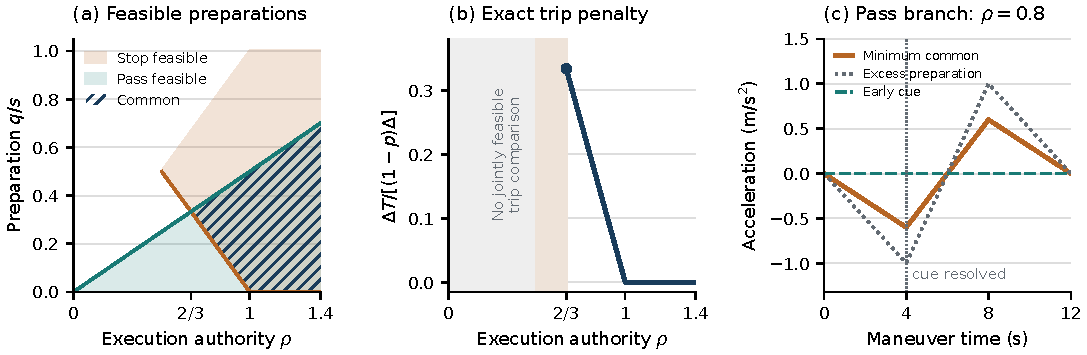
\includegraphics[width=0.90\textwidth]{fig2_preparation.pdf}
\renewcommand{\thefigure}{S1}
\caption{Closed-form maneuver in Proposition 1. The feasible stop/pass preparation intervals, normalized complete-trip information penalty, and passing-branch preparation profiles belong to the declared continuous three-node family. They are separate from the sampled LP and observed vehicle trajectories.}
\end{figure}

\FloatBarrier\stepcounter{section}\section*{F. COMFORT AND EXECUTOR TIMING EVALUATIONS}\setcounter{subsection}{0}

\subsection*{F.1. Training protocol and soft-regularizer trade-off}

The short-task adaptation used the previously validation-selected seed-7 actor; new critics were fitted during a shared 40000-step actor-frozen prefix. Branches A and B then each received 300000 integration steps. Final actor-update counts were 37610 and 37590, respectively, because terminal episodes can contain fewer than four integration steps per decision. Thus interaction budgets match, while optimizer invocation counts differ by 0.053\%. The recorded models are the fixed final checkpoints, not comfort-selected peaks. The executor comparison reuses these final actors without further training.

Under the original arrival cut, A and B had mean \(I_j\) 77.861 and 49.083, respectively, and mean trip times 270.389 and 302.500 s. The regularizer therefore lowered \(I_j\) by 36.96\% but increased time by 11.88\%, exceeding the development travel-time allowance. The worst jerk also rose rather than improving. These results motivated examination of execution feasibility; they do not show that all regularization weights or methods fail.

The original final traces contained 62 jerk-exceedance substeps (28 for A and 34 for B), all at states where the nominal jerk interval conflicted with a safety or nonnegative-speed bound. Twenty were associated with the low-/zero-speed bound. These counts refer to the original traces before adding terminal settling. The diagnostic identifies the conflicts in these records, rather than proving that every real-vehicle jerk spike has that cause.

An offline feasibility diagnostic considered all 25 stops in the completed and settled A/B traces. Over each final window of at most 12 s, it fixed the recorded initial state, endpoint position, endpoint time, and terminal zero speed/acceleration. Twenty-four admitted trajectories within the discrete acceleration and jerk bounds. One signal stop in A condition 7 was infeasible, independently confirmed by linear programming. This is an offline witness of available smoothing space in these events, not a deployable clairvoyant controller or 25 independent training repetitions.

\subsection*{F.2. Executor configurations and information access}

The three executor configurations use the same two fixed actors and nine development conditions. The complete configuration was selected after examining the earlier configurations on these conditions; no held-out executor confirmation set is available.

\begin{table}[!t]
\centering
\renewcommand{\thetable}{S2}
\caption{Executor configurations on the development conditions.}
\setlength{\tabcolsep}{3pt}
\renewcommand{\arraystretch}{1.12}
\begin{tabularx}{\textwidth}{@{}>{\hsize=0.774481\hsize\linewidth=\hsize\raggedright\arraybackslash}X>{\hsize=0.335312\hsize\linewidth=\hsize\centering\arraybackslash}X>{\hsize=1.795252\hsize\linewidth=\hsize\centering\arraybackslash}X>{\hsize=1.094955\hsize\linewidth=\hsize\raggedleft\arraybackslash}X@{}}
\toprule
\textbf{configuration} & \textbf{completed / 18} & \textbf{observed issue} & \textbf{interpretation} \\
\midrule
Initial backup & 17/18 & one red-light violation; fallback and jerk exceedances & initial construction failed \\
Target-type and signal handling & 18/18 & A maximum local overspeed 0.744 m/s versus 0.612 m/s baseline & exceeded the +0.1 m/s development allowance \\
Complete executor & 18/18 & no red-light, local-overspeed, physical, or fallback events observed & final development candidate \\
\bottomrule\end{tabularx}
\end{table}

The intermediate configuration distinguished positive speed targets from terminal rest and added a stop-or-clear test at green end. The complete configuration additionally incorporated the legal 80 km/h road cap rather than the original outer clamp. The executor reads the simulator-known signal schedule beyond the actor's broadcast range. Consequently, its total effect bundles feasibility, signal handling, information access, and road-limit enforcement. It must not be described as a controlled polynomial-only, jerk-only, or equal-information ablation. The observed absence of fallback in the complete configuration does not prove that its feasible set is nonempty in all states.

The final comparison uses discrete velocity and acceleration at the recorded 0.5 s resolution. Local overspeed is tested against the 35 km/h curve cap and 80 km/h road cap with a \(10^{-6}\) m/s tolerance. Legacy counters that omitted the local curve cap are not used for these claims.

\subsection*{F.3. All paired comfort conditions}

Conditions 0--2 use offsets 0, 30, and 60 s with warm SOC 0.85; conditions 3--5 use those offsets with cold SOC 0.90; conditions 6--8 use them with cold SOC 0.95. Initial speed is 16 m/s throughout. Percentages compare the complete executor with the original executor within each actor and condition. Positive \(I_j\) reduction is beneficial; positive time or energy change is an increase.

\begin{table}[!t]
\centering
\renewcommand{\thetable}{S3}
\caption{Complete paired development effects.}
\setlength{\tabcolsep}{3pt}
\renewcommand{\arraystretch}{1.12}
\begin{tabularx}{\textwidth}{@{}>{\hsize=0.833516\hsize\linewidth=\hsize\raggedright\arraybackslash}X>{\hsize=0.833516\hsize\linewidth=\hsize\centering\arraybackslash}X>{\hsize=1.101119\hsize\linewidth=\hsize\centering\arraybackslash}X>{\hsize=1.063830\hsize\linewidth=\hsize\centering\arraybackslash}X>{\hsize=1.168019\hsize\linewidth=\hsize\raggedleft\arraybackslash}X@{}}
\toprule
\textbf{actor} & \textbf{condition} & \textbf{\(I_j\) reduction \%} & \textbf{time change, s} & \textbf{energy change \%} \\
\midrule
A & 0 & 22.22 & +0.5 & -0.89 \\
A & 1 & 27.90 & +0.0 & -1.37 \\
A & 2 & 28.48 & +0.5 & -0.27 \\
A & 3 & 20.92 & +0.5 & -0.77 \\
A & 4 & 21.80 & -1.0 & -1.21 \\
A & 5 & 17.60 & +1.0 & -1.28 \\
A & 6 & 28.27 & -1.0 & -0.01 \\
A & 7 & 36.63 & +1.0 & -1.97 \\
A & 8 & 30.84 & -0.5 & -0.72 \\
B & 0 & 48.59 & -0.5 & -0.14 \\
B & 1 & 43.30 & +0.5 & -0.32 \\
B & 2 & 41.71 & +0.5 & -1.53 \\
B & 3 & 52.88 & -0.5 & -1.02 \\
B & 4 & 45.17 & +0.5 & -1.47 \\
B & 5 & 9.80 & +2.5 & +1.30 \\
B & 6 & 53.96 & -0.5 & -0.88 \\
B & 7 & 47.06 & +0.5 & -0.79 \\
B & 8 & 40.19 & +0.5 & -0.99 \\
\bottomrule\end{tabularx}
\end{table}

These eighteen pairs are deterministic condition responses from one training seed. They support the displayed finite-condition effects, not a seed-level confidence interval. There is no additional training-seed or held-out-condition confirmation for this comparison.

\subsection*{F.4. Acceleration diagnostics and endpoint conventions}

Acceleration RMS is computed per trip as \(\sqrt{\sum_k a_k^2\Delta t/T}\) and then averaged. Time below \(-2\) m/s\(^2\) is a post hoc descriptive threshold, not a regulatory or passenger-comfort standard.

\begin{table}[!t]
\centering
\renewcommand{\thetable}{S4}
\caption{Supplementary acceleration diagnostics.}
\setlength{\tabcolsep}{3pt}
\renewcommand{\arraystretch}{1.12}
\begin{tabularx}{\textwidth}{@{}>{\hsize=0.929195\hsize\linewidth=\hsize\raggedright\arraybackslash}X>{\hsize=1.000970\hsize\linewidth=\hsize\centering\arraybackslash}X>{\hsize=1.117362\hsize\linewidth=\hsize\centering\arraybackslash}X>{\hsize=0.952473\hsize\linewidth=\hsize\raggedleft\arraybackslash}X@{}}
\toprule
\textbf{actor / executor} & \textbf{mean acceleration RMS, m/s\(^2\)} & \textbf{largest braking magnitude, m/s\(^2\)} & \textbf{mean time below \(-2\) m/s\(^2\), s} \\
\midrule
A / original & 0.643 & 3.50 & 6.50 \\
A / complete executor & 0.618 & 3.50 & 6.94 \\
B / original & 0.514 & 3.50 & 5.33 \\
B / complete executor & 0.490 & 3.50 & 5.50 \\
\bottomrule\end{tabularx}
\end{table}

The benefit also survives the original arrival cut: A's \(I_j\) changes from \textbf{77.861 to 61.879}, a \textbf{20.53\%} reduction; B's changes from \textbf{49.083 to 32.205}, a \textbf{34.39\%} reduction. The larger settled-tail percentages use a different, explicitly matched denominator and must not be mixed with these values.

The principal metrics include safety interventions and terminal settling. The secondary cut reproduces the arrival-only convention. Both conventions show lower cumulative squared jerk, but the percentages differ. No metric silently omits an emergency segment or counts an incomplete route as a low-cost complete trip. Full paired trajectories belong to the identified experiment archives; this package retains their published condition summaries.

\begin{figure}[!t]
\centering
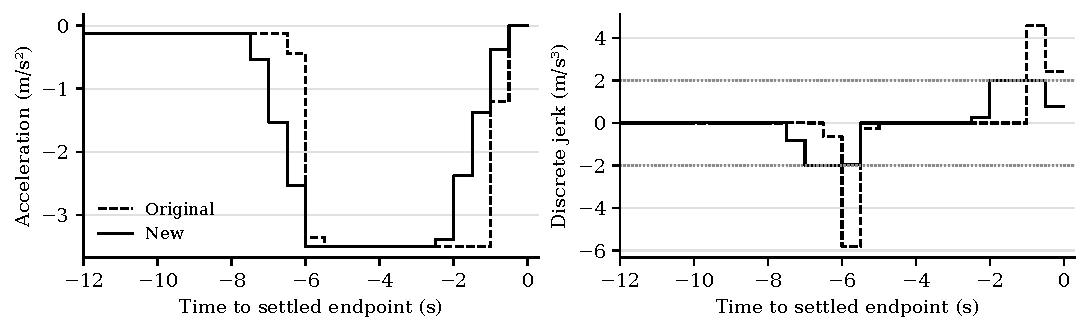
\includegraphics[width=0.90\textwidth]{fig_comfort_tail.pdf}
\renewcommand{\thefigure}{S2}
\caption{Actor A, condition 0, original versus complete executor. Actual acceleration and discrete jerk cover each trip's final 12 s and are aligned to its own settled endpoint. They illustrate different trajectories, not a same-state or fixed-clock causal comparison. Dotted lines indicate the configured jerk bounds. All paired condition effects remain in Table S3.}
\end{figure}

\subsection*{F.5. Timing-use intervention and fixed actor}

The experiment uses the final unregularized actor A from the short-task development seed. All six actor tensors are unchanged. The actor and its thirteen observation channels, including the original SPaT input, remain identical across arms. The executor updates every 0.5 s and the actor every 2 s in both arms. Signals follow the same realized schedule; withholding a countdown does not change the environment.

Both arms receive current color within 1000 m. Only the timing arm uses the remaining phase duration for the existing green-end stop-or-clear test. Current red-color stopping, curve and road limits, brake-release bounds and emergency handling are shared. Outside range, neither executor accesses signal color or timing, although both know the static signal location. The pure action-selection interface contains no global clock or offset. Ground-truth logging and same-state alternate-action diagnostics cannot alter the selected action.

The current-color arm uses reactive red-stop/green-pass execution. Unknown countdown is neither filled with an optimistic value nor replaced with a requirement that permanently prevents green passage. This arm is not claimed safe against an arbitrarily imminent unobserved phase change. The experiment measures the use of timing by this execution construction, conditional on an actor that already observes SPaT; it is not a whole-controller information ablation or a visual-perception test.

\subsection*{F.6. Timing conditions and metric definitions}

The three pack regimes are crossed with offsets 0, 30 and 60 s at initial speed 16 m/s. The primary metric is integrated squared actual jerk in the fixed 2200--3300 m signal window, assigning substeps by position midpoint. Full-trip energy, time, jerk, settled completion, red crossing, local overspeed, actuator violations and fallback are retained. Completion includes terminal settling under the same criteria as main Table III.

The intervention protocol was fixed before its outcomes. All nine pairs used the same actor without training updates. The color-only arm failed one condition, so there is no complete-route cost comparison over all nine pairs. The additional reporting conditions were not evaluated; the evidence is limited to these development conditions.

\subsection*{F.7. Every paired timing condition}

\begin{table}[!t]
\centering
\renewcommand{\thetable}{S5}
\caption{Signal-window squared jerk and completion. Values are in m\(^2\)/s\(^5\). The color-only value in condition 7 is an incomplete window and must not be treated as a matched completed-window cost. The last column compares complete raw trajectories, not merely rounded metrics.}
\setlength{\tabcolsep}{3pt}
\renewcommand{\arraystretch}{1.12}
\begin{tabularx}{\textwidth}{@{}>{\hsize=0.618047\hsize\linewidth=\hsize\raggedright\arraybackslash}X>{\hsize=0.964153\hsize\linewidth=\hsize\centering\arraybackslash}X>{\hsize=0.843634\hsize\linewidth=\hsize\centering\arraybackslash}X>{\hsize=1.384425\hsize\linewidth=\hsize\centering\arraybackslash}X>{\hsize=1.189740\hsize\linewidth=\hsize\raggedleft\arraybackslash}X@{}}
\toprule
\textbf{condition} & \textbf{current color} & \textbf{color + timing} & \textbf{settled: color / timing} & \textbf{trajectory relation} \\
\midrule
0 & 5.516 & 5.516 & yes / yes & identical \\
1 & 2.270 & 2.270 & yes / yes & identical \\
2 & 63.518 & 63.518 & yes / yes & identical \\
3 & 0.524 & 0.524 & yes / yes & identical \\
4 & 24.647 & 24.647 & yes / yes & identical \\
5 & 33.555 & 33.555 & yes / yes & identical \\
6 & 4.113 & 4.113 & yes / yes & identical \\
7 & 46.300 (partial) & 36.940 & no / yes & different \\
8 & 8.636 & 8.636 & yes / yes & identical \\
\bottomrule\end{tabularx}
\end{table}

The timing arm receives countdown in 1498 substeps and performs 466 green-end tests. These tests change the selected action in five substeps of condition 7; all other completed pairs have exactly identical recorded trajectories. No condition-level confidence interval is interpreted as independent training replication.

Unfinished trips remain in the raw records. The color-only failure ends at 182.0 s and x=3001.47 m, whereas timing completes the full route at 344.5 s. Comparing these as journey durations or averaging their unequal-length energy/jerk records does not establish a task-level benefit. The eight jointly completed pairs instead have zero energy, time and jerk differences.

\subsection*{F.8. Late-green event}

Condition 7 has SOC 0.95, temperature -10 \textdegree{}C and offset 30 s. At the first difference, t=177.5 s, both states have x=2914.128 m and v=20.280 m/s, with identical previous acceleration and actor command. Timing reads 2.5 s of remaining green and changes acceleration from 0.408 to 0.160 m/s\(^2\). At t=178.0 s it begins negative acceleration, then deepens braking within the jerk limit. The selected action is changed before the vehicle is unable to stop; subsequent actor commands can differ because the states have diverged.

Green ends at t=180.0 s. Current-color execution then has v=21.221 m/s and only 33.976 m to the line. Its stopping-distance lower bound, even with instantaneous maximum braking and no jerk restriction, is \(v^2/(2\times3.5)=64.335\) m. It invokes four emergency substeps, reaches a jerk magnitude of 7.738 m/s\(^3\), and crosses on red at t=181.898 s. Timing instead settles at x=2998 m at t=186.0 s and later completes the route, with no fallback and peak discrete jerk 2.000 m/s\(^3\).

This is a controlled event-level effect on the stated development conditions. It does not establish a general travel-cost reduction or a learned visual timing mechanism.

\FloatBarrier\stepcounter{section}\section*{G. VISUAL-DRIVING OUTCOMES AND LOCALIZATION}\setcounter{subsection}{0}

\subsection*{G.1. Evaluation conventions}

F/S/J use the evaluator with the true-position terminal command override removed. JH retains the rule setting cmd=0 at true x\textgreater=3999 m and v\textless=0.3 m/s. A source-hash-checked patch implements this protocol choice; it does not alter the learner, weights, memory, or termination tests. F/S/J logs contain 340 substeps meeting this state condition with nonzero commands, while all 77 matching JH substeps have zero commands. Consequently JH is reported separately and is excluded from matched F/S/J effects.

The companion reevaluation entry point requires an explicit seed, arm, and terminal protocol. Two seed-0, condition-0 checkpoint probes verify the distinction: F under the no-override path has T=240.5 s and R=-38.181836, while the override path gives T=240.0 s; JH under the override path has T=239.5 s and R=-37.235211, while removing the branch gives T=240.5 s and approximately R=-37.318192. These probes do not replace all 27 JH outcomes, and small cross-runtime numerical differences remain.

\subsection*{G.2. Every seed and arm}

\begin{table}[!t]
\centering
\renewcommand{\thetable}{S6}
\caption{All visual seed summaries, with the JH terminal convention identified. Mean R includes all nine attempts. I\_j, time, and energy condition on each row's own completions and must not be subtracted as matched effects. JH rows retain the terminal override; F/S/J rows use current no-override records. Units are as in main Table III.}
\setlength{\tabcolsep}{3pt}
\renewcommand{\arraystretch}{1.12}
\begin{tabularx}{\textwidth}{@{}>{\hsize=0.442105\hsize\linewidth=\hsize\raggedright\arraybackslash}X>{\hsize=0.589474\hsize\linewidth=\hsize\centering\arraybackslash}X>{\hsize=0.957895\hsize\linewidth=\hsize\centering\arraybackslash}X>{\hsize=1.178947\hsize\linewidth=\hsize\centering\arraybackslash}X>{\hsize=1.326316\hsize\linewidth=\hsize\centering\arraybackslash}X>{\hsize=1.252632\hsize\linewidth=\hsize\centering\arraybackslash}X>{\hsize=1.252632\hsize\linewidth=\hsize\raggedleft\arraybackslash}X@{}}
\toprule
\textbf{Seed} & \textbf{Mode} & \textbf{Completed n / 9} & \textbf{Mean R, all 9} & \textbf{Mean I\_j, completed} & \textbf{Time, completed} & \textbf{Energy, completed} \\
\midrule
0 & F & 9 & -40.265 & 99.238 & 220.556 & 628.351 \\
0 & S & 9 & -39.147 & 86.998 & 218.889 & 601.001 \\
0 & J & 9 & -40.622 & 98.563 & 222.167 & 634.682 \\
0 & JH & 9 & -39.081 & 92.333 & 217.778 & 601.643 \\
1 & F & 9 & -39.970 & 86.128 & 225.278 & 609.665 \\
1 & S & 9 & -38.874 & 80.026 & 217.944 & 595.525 \\
1 & J & 9 & -39.420 & 114.105 & 220.556 & 604.877 \\
1 & JH & 9 & -38.875 & 79.829 & 217.000 & 597.653 \\
2 & F & 6 & -48.105 & 107.194 & 234.333 & 646.271 \\
2 & S & 9 & -40.246 & 97.382 & 234.333 & 597.217 \\
2 & J & 8 & -44.263 & 149.347 & 248.500 & 674.051 \\
2 & JH & 7 & -44.400 & 150.506 & 243.571 & 642.908 \\
\bottomrule\end{tabularx}
\end{table}

The current F/S/J records remove a true-position terminal command override. All JH rows retain the terminal override, so their values are descriptive separate-protocol results rather than a uniform four-mode comparison. The same nine development conditions and one frozen detector are shared; three training seeds do not imply 27 independent environments.

\subsection*{G.3. Common-success contrasts}

\begin{table}[!t]
\centering
\renewcommand{\thetable}{S7}
\caption{Matched-protocol common-success contrasts relative to F. Every row uses the same condition IDs and terminal convention on both sides; R is conditional on that intersection. The JH outcomes remain in Table S6 and are not used for cross-version contrasts.}
\setlength{\tabcolsep}{3pt}
\renewcommand{\arraystretch}{1.12}
\begin{tabularx}{\textwidth}{@{}>{\hsize=1.066667\hsize\linewidth=\hsize\raggedright\arraybackslash}X>{\hsize=0.533333\hsize\linewidth=\hsize\centering\arraybackslash}X>{\hsize=2.285714\hsize\linewidth=\hsize\centering\arraybackslash}X>{\hsize=0.380952\hsize\linewidth=\hsize\centering\arraybackslash}X>{\hsize=0.914286\hsize\linewidth=\hsize\centering\arraybackslash}X>{\hsize=0.914286\hsize\linewidth=\hsize\centering\arraybackslash}X>{\hsize=0.990476\hsize\linewidth=\hsize\centering\arraybackslash}X>{\hsize=0.914286\hsize\linewidth=\hsize\raggedleft\arraybackslash}X@{}}
\toprule
\textbf{Contrast} & \textbf{Seed} & \textbf{Condition IDs} & \textbf{n} & \textbf{Delta I\_j} & \textbf{Delta time} & \textbf{Delta energy} & \textbf{Delta R} \\
\midrule
S - F & 0 & 0,1,2,3,4,5,6,7,8 & 9 & -12.240 & -1.667 & -27.350 & +1.118 \\
S - F & 1 & 0,1,2,3,4,5,6,7,8 & 9 & -6.101 & -7.333 & -14.140 & +1.096 \\
S - F & 2 & 0,1,3,4,6,7 & 6 & +4.144 & +15.167 & -41.915 & +0.296 \\
J - F & 0 & 0,1,2,3,4,5,6,7,8 & 9 & -0.674 & +1.611 & +6.331 & -0.357 \\
J - F & 1 & 0,1,2,3,4,5,6,7,8 & 9 & +27.977 & -4.722 & -4.788 & +0.550 \\
J - F & 2 & 1,3,4,6,7 & 5 & +45.832 & +13.900 & +9.343 & -1.448 \\
\bottomrule\end{tabularx}
\end{table}

Each intersection is selected by both policies completing the trip, so these are conditional descriptive contrasts. The primary functional outcomes remain completion, violations, progress, and actual jerk. No cross-version JH/F contrast is interpreted as a training effect. S completes all attempts but its seed-2 matched subset has higher jerk integral and longer travel time; functional visual dependence does not require a consistent encoder-update advantage.

\subsection*{G.4. Event and metric definitions}

All twelve offline Z probes report 0.98305; their held-out portion has 59 sequences, giving 58/59. Renderer-projected ROI and association metadata are used for this diagnostic, whereas deployment uses predicted ROI. The value is therefore not deployed closed-loop detector accuracy. A logged encoder\_grad after a combined critic-plus-supervision backward pass is a total gradient norm, not a pure TD gradient.

Trajectory analysis places four high-speed signal violations at yellow-onset states with distance below the ideal stopping bound v\^{}2/7: (d,v) approximately (3.5,19.3), (16.1,16.2), (45.9,22.2), and (13.8,22.2) in meters and m/s. The last two belong to legacy JH. One J violation is low-speed red crossing; one F trip remains approximately 6 m before the line, with 884 stationary pre-step samples and 300 true-green/retained-nongreen samples. The stopping bound excludes recovery from those high-speed onset states, not earlier prevention.

Signal phase is logged at substep start t0. The recorded crossing\_speed field is v0 of that substep; exact crossing speed requires within-step kinematics.

Cue-removal probes change both the frozen perception path and the policy representation, supporting system dependence on visual cues without isolating Z. The constant-command v4r reference completes nine conditions without signal or curve-speed violations, with I\_j=100.954 and peak jerk=12.2 m/s\^{}3. It has rounded records and incomplete evaluation identity, so it remains descriptive.

Intervention frequency does not measure the fraction of decisions in which commands have no effect. The report's per-episode mean intervention percentages and pooled-substep percentages use different denominators; the latter are 89.14\%, 95.28\%, 91.87\%, and 87.23\% for F/S/J/legacy JH. Neither coarse conditioning on first applied action and speed nor a small correlation establishes absence of command effects.

\subsection*{G.5. Nine S override episodes}

For P-V, the first nonzero trajectory jerk-override flag is matched to its pre-step layer record. All nine episodes have an earlier accepted lamp color; this does not imply that subsequent colors remain correct. The categories below describe observed first-event contexts, not counterfactual benefits of an untested fix.

\begin{table}[!t]
\centering
\renewcommand{\thetable}{S8}
\caption{Every affected S episode. Seeds 0/1/2 denote the three reported policies. Values are at the first override's pre-step state; positions and velocities are rounded. The signal-terminal label here is a contextual category, distinct from the below-5 m/s P-B threshold.}
\setlength{\tabcolsep}{3pt}
\renewcommand{\arraystretch}{1.12}
\begin{tabularx}{\textwidth}{@{}>{\hsize=0.828744\hsize\linewidth=\hsize\raggedright\arraybackslash}X>{\hsize=0.947137\hsize\linewidth=\hsize\centering\arraybackslash}X>{\hsize=0.633260\hsize\linewidth=\hsize\centering\arraybackslash}X>{\hsize=0.556167\hsize\linewidth=\hsize\centering\arraybackslash}X>{\hsize=2.034692\hsize\linewidth=\hsize\raggedleft\arraybackslash}X@{}}
\toprule
\textbf{Seed / condition} & \textbf{First adopted color} & \textbf{Position, m} & \textbf{Speed, m/s} & \textbf{First-event context} \\
\midrule
0 / 0 & red & 2984.7 & 5.34 & Signal-terminal stop \\
0 / 2 & green & 3992.5 & 14.27 & Endpoint handling \\
0 / 5 & green & 2988.9 & 22.22 & Perceived red during true green \\
0 / 8 & green & 3992.7 & 13.80 & Endpoint handling \\
2 / 3 & red & 2986.0 & 5.31 & Signal-terminal stop \\
2 / 5 & green & 2988.2 & 22.22 & Perceived yellow during true green \\
2 / 6 & red & 2986.9 & 5.80 & Signal-terminal stop \\
2 / 7 & yellow & 2910.2 & 13.74 & Range update with positive command \\
2 / 8 & green & 3985.8 & 13.19 & Endpoint handling \\
\bottomrule\end{tabularx}
\end{table}

The three endpoint execution targets lie at about 4056.0, 4049.3, and 4040.0 m. Memory's raw endpoint ranges are 48.53, 41.66, and 39.25 m at those states; the target additionally includes the 15 m endpoint bias. Thus the entire target extension beyond the 4000 m route cannot be assigned to image measurement error.

For condition 5 in seeds 0 and 2, the original layer record confirms true green at the event while memory reports red or yellow. Both occur at 147.5 s using the same condition camera stream. The preceding green confidence is high; the 8 m color-freeze rule does not yet suppress the update around 11 m. Each produces -3.5 m/s\(^2\) braking without a recorded red crossing. This is a concrete near-line perception failure mode, but changing the freeze distance has not been evaluated and could suppress a valid red observation.

Seed 2 condition 7 has an inward distance revision during approach while the policy requests positive acceleration toward a nonpassable signal. Its target and command context distinguish it from late first recognition. The three signal-terminal episodes involve low-speed stopping near the buffered point. The full-trip peak for S is 10 m/s\(^3\) at \(x=2993.15\) m and \(v=1.5\) m/s in seed 2 condition 3; F's peak is 12.144 m/s\(^3\) at \(x=2988.27\) m and \(v=17.17\) m/s in seed 0 condition 4, with perceived yellow during true green. Peak magnitude alone therefore does not measure anticipation quality.

\FloatBarrier\stepcounter{section}\section*{H. PREPARATION BRANCHES AND TARGET-UPDATE DIAGNOSIS}\setcounter{subsection}{0}

\subsection*{H.1. Frozen-state design and output gating}

The short-branch study freezes an approach to the signal at 3000 m before it enters the 200 m visibility range. The first state is at time 136 s, position 2746.805 m, speed 22.222 m/s, and zero acceleration. The second is at time 141 s, position 2746.361 m, speed 16 m/s, and zero acceleration. For the second state, an execution speed ceiling of 16 m/s was imposed from 2400 m; the actor's normalization was unchanged. Sensor history, event memory, and random streams are cloned from each frozen state. No signal track exists at freezing.

The stopping scene starts in red and changes to green 50 s after freezing. The passing scene starts with a 30 s green phase. Each state uses a constant normalized command \(u=1\) and three frozen supervised-representation policies, jerk limits 2/3/4 m/s\(^3\), and early phase adoption or two delayed preparation rules. The feasibility-triggered rule retains the existing stopping-backup constraint but omits the unknown-light comfort envelope. The conservative rule additionally applies that envelope. Neither is asserted to optimize the theoretical comparison. The code names are \path{min} and \path{cons}, respectively.

Higher-speed target adoption distances are 150, 120, 100, 89, 78, 67, 56, and 44 m; the lower-speed group additionally includes 32 m. The corresponding sizes are \(4\times2\times3\times(1+2\times8)=408\) and \(4\times2\times3\times(1+2\times9)=456\). These are factorial branches from two approach states. They are not 864 independently sampled routes, and the three policies do not constitute new training replications.

The phase output is opened when position reaches the target plus a nominal \(0.5v_0\) lead distance. Before that point, lamp-color probabilities are removed, and a colorless-track option allows detection geometry to create an unknown-phase track. The detector still sees colored pixels; the policy encoder does too. The nominal 0.5 s allowance is not a measured adoption delay shared by all branches: 804/816 delayed branches adopt in the same recorded instant as output opening, and 12/816 do so 0.5 s later. The next execution substep is a separate clock.

The intervention is an output gate, not image-level occlusion. A separate dark-lamp detector candidate had an off-class rate of 0.905 but completed only 6/9 normal-visibility probe conditions with one signal violation; it was excluded. The branch results use the original detector and do not establish occlusion robustness or a learned Z timing mechanism.

\subsection*{H.2. Information histories before adoption}

The explicit phase mask works: all hidden records have phase unknown and no reported detector color. It does not remove scene-dependent detection confidence, tracking onset, or range estimates. Comparing stop/pass branches while both remain hidden gives Table S9. All constant commands are identical; applied accelerations need not be.

\begin{table}[!t]
\centering
\renewcommand{\thetable}{S9}
\caption{Residual scene distinctions in delayed constant-command pairs. Differences are checked at equal absolute times while both phase outputs remain hidden, with numerical tolerance \(10^{-8}\). A pair is counted once if any such difference occurs.}
\setlength{\tabcolsep}{3pt}
\renewcommand{\arraystretch}{1.12}
\begin{tabularx}{\textwidth}{@{}>{\hsize=0.995012\hsize\linewidth=\hsize\raggedright\arraybackslash}X>{\hsize=0.498753\hsize\linewidth=\hsize\centering\arraybackslash}X>{\hsize=1.014963\hsize\linewidth=\hsize\centering\arraybackslash}X>{\hsize=1.099751\hsize\linewidth=\hsize\centering\arraybackslash}X>{\hsize=1.391521\hsize\linewidth=\hsize\raggedleft\arraybackslash}X@{}}
\toprule
\textbf{Speed / preparation} & \textbf{Pairs} & \textbf{Track-onset differences} & \textbf{Range-history differences} & \textbf{Applied-acceleration differences} \\
\midrule
22.2 / min & 24 & 24 & 24 & 10 \\
22.2 / cons & 24 & 24 & 24 & 24 \\
16 / min & 27 & 27 & 27 & 6 \\
16 / cons & 27 & 27 & 27 & 15 \\
\bottomrule\end{tabularx}
\end{table}

For example, at 22.2 m/s, jerk 2, conservative preparation, and target adoption 67 m, the stopping track is established 3.0 s after freezing, before the passing track. At 3.5 s, both phases remain hidden, yet the applied accelerations are \(-1\) and \(0\) m/s\(^2\). The branch identifiers are \path{99bce1c256d1} and \path{ea5b8d6e5ad9}. Their physical states agree before the first track difference.

The 55/102 pairs with different pre-resolution applied accelerations do not satisfy the common-prefix condition imposed by the LP. Even pairs with the same observed actions do not demonstrate identical information histories. For the learned-policy branches, colored image inputs additionally remain in Z. These facts prevent treating the intervention as pure loss of an early visual distinction.

\subsection*{H.3. Completion, recovery, and fixed-endpoint cost}

All 864 branches complete the short segment, and no signal violation is recorded. All 432 stopping branches record a stop before the line. However, 200 branches contain emergency jerk overrides over their full duration, with a maximum observed jerk of 12.2 m/s\(^3\). These branches are not witnesses of feasibility under their nominal jerk limit.

The primary response criterion uses every speed in the approach: from freezing until the first stop within 60 m before the line, or line crossing. It requires neither fallback nor jerk override. A branch passing this criterion has not thereby passed a passenger-comfort test. The full-branch override count is reported separately because later restart and passage can also require recovery.

\begin{table}[!t]
\centering
\renewcommand{\thetable}{S10}
\caption{All frozen-policy branch groups. S0/S1/S2 denote the three archived supervised policies; they retain colored image inputs. Counts include stopping and passing scenes and all attempted information/jerk settings. The full-approach criterion and full-branch jerk-override count use different temporal windows.}
\setlength{\tabcolsep}{3pt}
\renewcommand{\arraystretch}{1.12}
\begin{tabularx}{\textwidth}{@{}>{\hsize=0.963076\hsize\linewidth=\hsize\raggedright\arraybackslash}X>{\hsize=0.592662\hsize\linewidth=\hsize\centering\arraybackslash}X>{\hsize=1.186971\hsize\linewidth=\hsize\centering\arraybackslash}X>{\hsize=0.837959\hsize\linewidth=\hsize\centering\arraybackslash}X>{\hsize=1.484948\hsize\linewidth=\hsize\centering\arraybackslash}X>{\hsize=1.341722\hsize\linewidth=\hsize\centering\arraybackslash}X>{\hsize=0.592662\hsize\linewidth=\hsize\raggedleft\arraybackslash}X@{}}
\toprule
\textbf{Initial speed} & \textbf{Policy} & \textbf{Completed / attempted} & \textbf{Signal violations} & \textbf{Full approach without recovery} & \textbf{Branches with jerk override} & \textbf{Peak jerk} \\
\midrule
22.2 & constant & 102/102 & 0 & 67 & 24 & 12.200 \\
22.2 & S0 & 102/102 & 0 & 60 & 29 & 12.026 \\
22.2 & S1 & 102/102 & 0 & 73 & 20 & 11.333 \\
22.2 & S2 & 102/102 & 0 & 67 & 24 & 12.192 \\
16 & constant & 114/114 & 0 & 94 & 18 & 12.200 \\
16 & S0 & 114/114 & 0 & 79 & 32 & 12.187 \\
16 & S1 & 114/114 & 0 & 77 & 35 & 12.159 \\
16 & S2 & 114/114 & 0 & 94 & 18 & 12.170 \\
\bottomrule\end{tabularx}
\end{table}

Speed-restricted sensitivity checks give 731/864 without recovery at speeds at least 5 m/s and 761/864 at speeds at least 10 m/s, with 30 differing classifications. The full-approach count is 611/864. For the higher-speed constant conservative stopping branches, the counts are 16/24 over the full approach, 16/24 at 5 m/s, and 24/24 at 10 m/s. Main Table VII uses the full-approach outcome; both speed-restricted counts are secondary sensitivity summaries.

The simulator stops each branch at the first substep endpoint beyond 3300 m, producing unequal overshoot distances. Main Table VII therefore uses the exact crossing time inside the last substep. If \(x_k<3300\le x_{k+1}\), its duration \(\tau\in[0,\delta t]\) solves

\[3300-x_k=v_k\tau+\tfrac12a_k\tau^2.\tag{H1}\]

The reconstructed crossing is used only when both recorded velocity and trapezoidal position increments satisfy this constant-acceleration step. Those conditions hold for all constant-command passing branches. For example, at 22.2 m/s, jerk 3, and min target 67 m, the stored integer-step time difference is zero, while the common-endpoint difference is 0.05283 s. Thus equal rounded durations do not establish zero extra cost. Recorded energy differences remain tied to their actual segment endpoints and are not silently interpolated into exact matched-route energy.

\begin{figure}[!t]
\centering
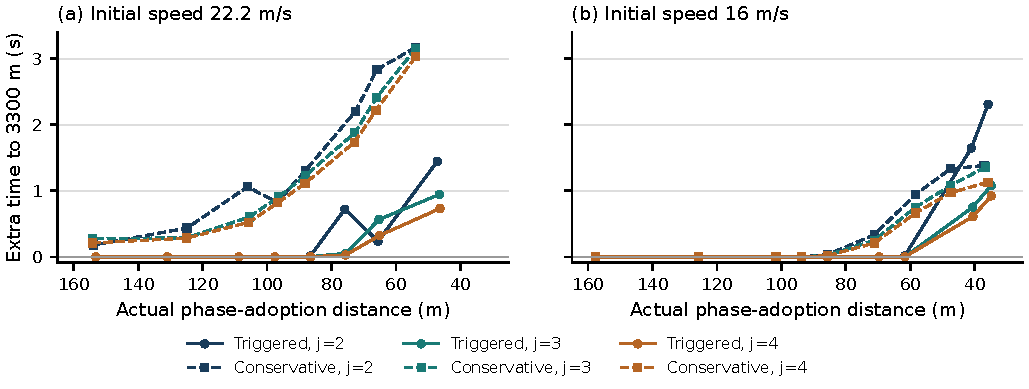
\includegraphics[width=0.90\textwidth]{fig_phase_cost.pdf}
\renewcommand{\thefigure}{S3}
\caption{Constant-command passing branches, with actual memory-adoption distance on the horizontal axis and extra time to the common 3300 m endpoint on the vertical axis. Curves connect the tested targets for readability; they do not assert monotonicity between settings. Feasibility-triggered and conservative preparation are shown separately for jerk 2/3/4. Each point is one frozen-state branch, not a sample mean. No LP boundary is overlaid because the resolution clock and cost criterion differ.}
\end{figure}

\subsection*{H.4. Recovery transitions and model limits}

\begin{table}[!t]
\centering
\renewcommand{\thetable}{S11}
\caption{Observed higher-speed recovery transitions in constant-command min branches. Here higher-speed explicitly means at least 10 m/s and remains secondary to Table VII's full-approach criterion. Adjacent entries are tested settings, not a proved monotone threshold. Both actual distances are taken from the stopping branch's memory-adoption time. They are not relabeled as LP zero-cost boundaries.}
\setlength{\tabcolsep}{3pt}
\renewcommand{\arraystretch}{1.12}
\begin{tabularx}{\textwidth}{@{}>{\hsize=0.858221\hsize\linewidth=\hsize\raggedright\arraybackslash}X>{\hsize=0.528136\hsize\linewidth=\hsize\centering\arraybackslash}X>{\hsize=1.346746\hsize\linewidth=\hsize\centering\arraybackslash}X>{\hsize=1.090223\hsize\linewidth=\hsize\centering\arraybackslash}X>{\hsize=1.086451\hsize\linewidth=\hsize\centering\arraybackslash}X>{\hsize=1.090223\hsize\linewidth=\hsize\raggedleft\arraybackslash}X@{}}
\toprule
\textbf{Initial speed} & \textbf{Jerk} & \textbf{Previous no-recovery target, m} & \textbf{Its actual adoption, m} & \textbf{First recovery target, m} & \textbf{Its actual adoption, m} \\
\midrule
22.2 & 2 & 89 & 97.688 & 78 & 86.824 \\
22.2 & 3 & 89 & 97.639 & 78 & 86.653 \\
22.2 & 4 & 89 & 97.639 & 78 & 86.622 \\
16 & 2 & 67 & 69.639 & 56 & 61.642 \\
16 & 3 & 56 & 61.639 & 44 & 45.935 \\
16 & 4 & 56 & 61.639 & 44 & 45.825 \\
\bottomrule\end{tabularx}
\end{table}

At 16 m/s and jerk 2, the first affected branch adopts at 61.642 m, whereas the previous tested branch adopts at 69.639 m without higher-speed recovery. Comparing 61.642 m with the LP's nominal 48 m zero-penalty grid coordinate gives 13.642 m, exceeding an 8 m frame distance. More fundamentally, this numerical difference compares a selected rule's recovery event with an optimal LP objective under a different clock; it is not a valid prediction error. No universal one-frame boundary agreement is claimed.

The latest closed-loop targets also do not cross all LP common-feasibility limits. At the higher speed, the target scan ends at 44 m; the LP's latest feasible nominal coordinates are about 22/11/0 m. A rule's fallback does not prove absence of another common feasible preparation. Conservative passing costs where the LP optimum is zero can reflect overpreparation, consistent with the distinction in (E11), but cannot be assigned quantitatively to that equation for this different executor.

\subsection*{H.5. Record timing and event selection}

The analysis reuses all 864 P-B records and all 27 S evaluations in P-V. The first accepted phase defines \(t_{\rm info}\): memory must report seen and a red, yellow, or green phase. Unknown and off are excluded. This does not use simulator truth to select adoption. In all 432 stopping branches it agrees with the original truth-correct adoption timestamp; in 408/432 a stopping target already exists before that time.

P-B records contain post-substep state and subsequently updated memory. A fallback/jerk flag in record \(k\) describes the action executed from the preceding state, before the image update stored in record \(k\). Event-trigger checks therefore use record \(k-1\). Range innovations end at \(k-1\); including \(k\) would mix an observation received after the trigger with its cause. P-V layer logs contain pre-substep state and memory; previous acceleration is aligned from the original trajectory. The conventions are not merged into an artificial common timestamp.

The P-B event is the first fallback or jerk override strictly after adoption and through the first stop or crossing. A stop endpoint requires \(v<0.05\) m/s within 2940--3005 m; a crossing endpoint has \(x\ge3000\) m. This gives 195 events. Including adoption and earlier approach samples gives 197; the 200 full-branch jerk-override count additionally differs in window and event definition.

The source base \path{curve_layer.py} has SHA-256 \path{3c20801fa67df955dc85aa314a620d5cfd8ae6320a0cb64eb66fe034eb5764a0} in both P-C and P-V. The same routine, parameterized by the branch jerk, computes all backups below. This establishes base identity, not equal wrappers, information access, or policy states.

\subsection*{H.6. Target margins at adoption}

True-line distance is \(3000-x\), estimated-line distance is memory's \(\widehat d\), and the active visual signal target uses \(B(\widehat d)=\max(0.85\widehat d-6,0)\). Subtract the same \(D_\kappa(v,a;0)\) from each. In P-V, target positions are read from the layer log; a missing target is not assigned zero margin. A hold-at-rest target, when present, must be distinguished from the buffered signal target.

\begin{table}[!t]
\centering
\renewcommand{\thetable}{S12}
\caption{Adoption margins and subsequent outcomes. Distances are metres. P-B ranges use all stopping branches. P-V target values use the 18 initially nonpassable episodes; the other nine initially green episodes have no stopping target at adoption. P-V episode overrides are not assigned to that initial event.}
\setlength{\tabcolsep}{3pt}
\renewcommand{\arraystretch}{1.12}
\begin{tabularx}{\textwidth}{@{}>{\hsize=0.722892\hsize\linewidth=\hsize\raggedright\arraybackslash}X>{\hsize=0.444856\hsize\linewidth=\hsize\centering\arraybackslash}X>{\hsize=0.817424\hsize\linewidth=\hsize\centering\arraybackslash}X>{\hsize=1.012048\hsize\linewidth=\hsize\centering\arraybackslash}X>{\hsize=1.718258\hsize\linewidth=\hsize\centering\arraybackslash}X>{\hsize=1.284523\hsize\linewidth=\hsize\raggedleft\arraybackslash}X@{}}
\toprule
\textbf{Cohort} & \textbf{N} & \textbf{True-line margin} & \textbf{Estimated-line margin} & \textbf{Actual stopping-target margin} & \textbf{Outcome count} \\
\midrule
P-B, 22.2 m/s & 204 & 10.44--111.15 & 11.89--112.89 & -1.59--84.08; 12 negative & 111 later approach events \\
P-B, 16 m/s & 228 & 5.78--140.16 & 5.16--158.38 & -7.11--123.53; 19 negative & 84 later approach events \\
P-V, S & 27 & 87.98--102.55 & 35.59--106.14 & 11.52--71.50 for 18; missing for 9 & 9 episode overrides \\
\bottomrule\end{tabularx}
\end{table}

All 432 unbuffered line margins and release reserves are positive. Release ranges are 10.98--22.22 and 8.66--16.00 m/s at the two P-B speeds, and 21.82--22.22 m/s for P-V at adoption. Buffering and checks before color adoption strongly shape these positive line margins. The actual buffered target has negative margin in 31 branches, all min, and margin below 5 m in 53. The thresholds describe this development set; they do not define a probabilistic safety certificate.

\subsection*{H.7. Actual-delay LP references and residuals}

For each delayed constant-command passing branch, \(t_{200}\) is the exact crossing of \(x=2800\) m, calculated inside the recorded constant-acceleration substep. The frozen state about 253 m before the line is not the origin. Delay is \(t_{\rm info}-t_{200}\), including any early slowing by conservative preparation. Passing-time differences use the common 3300 m endpoint and the corresponding early branch.

The primary reference is the lower half-second LP grid point. Lowering the information delay relaxes common-prefix constraints. Lemma 2 orders the total optimum; in all feasible computed optima, the stopping branch binds its line constraint, so its loss is constant and the passing-branch reference inherits that ordering on the grid. This component property is not inferred from total-cost monotonicity alone. It does not equate fixed-horizon lost progress with full vehicle travel time.

\begin{table}[!t]
\centering
\renewcommand{\thetable}{S13}
\caption{Passing cost and LP-reference residuals. All ranges are seconds. Floor residuals exist for all 102 rows. Interpolation is secondary and has one unavailable value because its upper program is infeasible.}
\setlength{\tabcolsep}{3pt}
\renewcommand{\arraystretch}{1.12}
\begin{tabularx}{\textwidth}{@{}>{\hsize=0.903495\hsize\linewidth=\hsize\raggedright\arraybackslash}X>{\hsize=1.264893\hsize\linewidth=\hsize\centering\arraybackslash}X>{\hsize=0.555997\hsize\linewidth=\hsize\centering\arraybackslash}X>{\hsize=1.142573\hsize\linewidth=\hsize\centering\arraybackslash}X>{\hsize=0.906275\hsize\linewidth=\hsize\centering\arraybackslash}X>{\hsize=1.237093\hsize\linewidth=\hsize\centering\arraybackslash}X>{\hsize=0.989674\hsize\linewidth=\hsize\raggedleft\arraybackslash}X@{}}
\toprule
\textbf{Initial speed} & \textbf{Rule} & \textbf{N} & \textbf{Observed difference} & \textbf{Floor residual} & \textbf{Interpolated residual} & \textbf{Finite interpolation} \\
\midrule
22.2 m/s & Feasibility-triggered & 24 & 0.000--1.447 & 0.000--0.837 & 0.000--0.761 & 24 \\
22.2 m/s & Conservative & 24 & 0.180--3.173 & 0.180--2.225 & 0.180--2.149 & 23 \\
16 m/s & Feasibility-triggered & 27 & 0.000--2.309 & 0.000--2.117 & 0.000--2.026 & 27 \\
16 m/s & Conservative & 27 & 0.000--1.383 & 0.000--1.309 & 0.000--1.260 & 27 \\
\bottomrule\end{tabularx}
\end{table}

All 102 floor and 101 finite interpolated residuals are nonnegative in these records. Interpolation is not an LP optimum at a fractional delay. The upper-grid reference is not a lower bound; a negative upper-grid residual is therefore not a counterexample to the floor ordering.

\begin{table}[!t]
\centering
\renewcommand{\thetable}{S14}
\caption{Two bracketing cases. Detailed branch values are retained in lp\_reference\_decomposition.csv. The second row has an available floor reference, not a missing or zero cost.}
\setlength{\tabcolsep}{3pt}
\renewcommand{\arraystretch}{1.12}
\begin{tabularx}{\textwidth}{@{}>{\hsize=1.305949\hsize\linewidth=\hsize\raggedright\arraybackslash}X>{\hsize=0.558074\hsize\linewidth=\hsize\centering\arraybackslash}X>{\hsize=0.776204\hsize\linewidth=\hsize\centering\arraybackslash}X>{\hsize=0.745042\hsize\linewidth=\hsize\centering\arraybackslash}X>{\hsize=0.807365\hsize\linewidth=\hsize\centering\arraybackslash}X>{\hsize=1.807365\hsize\linewidth=\hsize\raggedleft\arraybackslash}X@{}}
\toprule
\textbf{Case} & \textbf{Actual delay, s} & \textbf{Observed difference, s} & \textbf{Lower LP reference, s} & \textbf{Upper LP reference, s} & \textbf{Consequence} \\
\midrule
22.2 m/s, min, jerk 2, target 56 m & 6.106228 & 0.236290 & 0.095978 & 0.317182 & Upper residual -0.080892 s; not a lower-bound test \\
22.2 m/s, cons, jerk 2, target 44 m & 8.106228 & 3.173047 & 1.419038 & Infeasible at 8.5 s & Floor available; no interpolation \\
\bottomrule\end{tabularx}
\end{table}

The first row's interpolated reference is 0.142974 s and residual 0.093316 s. The signed reference residual in main (19) is not the nonnegative within-model rule excess in main (17). Position-triggered output gating, scene-dependent geometry, different targets and endpoints, and emergency actions prevent transferring a general lower-bound guarantee between models.

\subsection*{H.8. State-fixed target substitutions}

The 71 selected post-adoption events at speed at least 5 m/s split into 31 with negative target margin at adoption and 40 with nonnegative adoption margin. The selected events in the first group occur one substep after adoption, but 16 branches already became infeasible earlier. A strictly post-adoption event is not necessarily the first trigger. Section H.9 aligns the update that first exhausts the margin and the immediately following physical response.

The 124 selected events below 5 m/s aggregate 92 freeze-crossing cases and 32 creeping cases. Their pooled position median is not used as a characteristic event location; the subclasses and trigger states are reported separately in Section H.9. S policies contribute 109/324 low-speed first events, compared with 15/108 for the constant policy; the higher-speed counts are 46/324 and 25/108. These descriptive denominators are condition branches, not independent roads or independent detector trainings. The same initial conditions do not force learned and constant policies to visit identical later states.

At all 195 preceding states, release and true-line backup remain feasible while the buffered-target margin is negative. The following static check isolates the effect of the target supplied to the base routine. It does not run a vehicle or change an archived policy.

\textbf{Algorithm 2 --- Offline target-trigger diagnosis.}

\begin{enumerate}
\def\labelenumi{\arabic{enumi}.}
\tightlist
\item
  Find adoption and the first strictly subsequent event within the declared approach window.
\item
  Retrieve the physical state and memory preceding its triggering action.
\item
  Evaluate \(D_\kappa\), the true-line, estimated-line, and actual buffered-target margins.
\item
  With that state, branch jerk, backup routine, and free-road cap fixed, call the single-target interval routine for each of the three target distances.
\item
  Record the returned reason and interval, then classify the event by speed and location. Evaluate range innovations only before the triggering action.
\end{enumerate}

\begin{table}[!t]
\centering
\renewcommand{\thetable}{S15}
\caption{State-fixed single-target substitutions. Each row uses the same 195 event-preceding states. The caps are the corresponding 22.2 or 16 m/s free-road speeds; protocol envelopes, other targets, and future observations are not re-simulated. Truth is an offline reference only.}
\setlength{\tabcolsep}{3pt}
\renewcommand{\arraystretch}{1.12}
\begin{tabularx}{\textwidth}{@{}>{\hsize=1.259603\hsize\linewidth=\hsize\raggedright\arraybackslash}X>{\hsize=0.417219\hsize\linewidth=\hsize\centering\arraybackslash}X>{\hsize=1.323179\hsize\linewidth=\hsize\raggedleft\arraybackslash}X@{}}
\toprule
\textbf{Target supplied to interval routine} & \textbf{Nonempty / 195} & \textbf{Returned outcome} \\
\midrule
Actual buffered signal target & 0 & 195 stop-distance infeasibility markers \\
Unbuffered estimated line & 195 & 195 feasible intervals \\
True physical line & 195 & 195 feasible intervals \\
\bottomrule\end{tabularx}
\end{table}

This diagnostic establishes a local target-dependent exclusion, not the trajectory benefit of deleting measurement protection. The buffer affects which target is required; removing it can admit actions that are unsafe under unknown line-position error. It also does not constitute a whole-executor equal-information ablation.

Across the pre-trigger windows, the per-branch maximum absolute range innovation has median 6.657 m and maximum 15.609 m. It combines prediction, fusion, and numerical propagation. Section D.2 gives the fixed-state relation used to distinguish these effects; the observed extrema are not future error bounds.

\subsection*{H.9. Trigger-aligned propagation, update, and response}

The trigger-aligned calculation reads the original P-B substep fields, independently evaluates the backup, and locates the memory update preceding the selected response. For the 31 adoption-negative branches it instead traces the first negative target margin up to adoption: 15 occur at adoption, 10 one substep earlier, and six three substeps earlier. For the remaining 164 branches it uses the update immediately before the selected post-adoption event. Each row records these two indices separately.

\begin{table}[!t]
\centering
\renewcommand{\thetable}{S16}
\caption{Exhaustion of propagated margin and actual response. Counts partition the 195 diagnostic branches. The final column counts jerk-limit exceedances in the physical response immediately following the identified update, with acceleration differences taken between adjacent records. Creeping is a separate diagnostic class. The original terminal class uses speed at the selected post-adoption event, not at the earlier trigger.}
\setlength{\tabcolsep}{3pt}
\renewcommand{\arraystretch}{1.12}
\begin{tabularx}{\textwidth}{@{}>{\hsize=1.680000\hsize\linewidth=\hsize\raggedright\arraybackslash}X>{\hsize=0.400000\hsize\linewidth=\hsize\centering\arraybackslash}X>{\hsize=0.960000\hsize\linewidth=\hsize\centering\arraybackslash}X>{\hsize=0.960000\hsize\linewidth=\hsize\raggedleft\arraybackslash}X@{}}
\toprule
\textbf{Update class} & \textbf{Branches} & \textbf{Nonnegative propagated margin} & \textbf{Immediate jerk exceedance} \\
\midrule
First negative margin at adoption & 15 & 15 & 11 \\
First negative margin before adoption & 16 & 16 & 11 \\
Other higher-speed inward update & 36 & 36 & 3 \\
Higher-speed, already negative after propagation & 4 & 0 & 4 \\
Terminal distance-freeze crossing & 92 & 92 & 70 \\
Creeping propagation discrepancy & 32 & 32 & 0 \\
\bottomrule\end{tabularx}
\end{table}

In 191/195 rows the update consumes a previously nonnegative propagated margin; four already have negative propagated margin. All targets in this arithmetic check are unclipped, and the maximum residual of main (13) is \(1.34\times10^{-14}\) m. Removing the creeping class leaves 159/163 such margin-exhaustion cases. This is a fixed-state arithmetic attribution; it does not imply that removing the update would preserve future closed-loop feasibility.

All 92 freeze-crossing cases have previous recorded range 17.7--23.6 m and updated range 8.9--14.2 m. The original memory tests the propagated pre-fusion range against 15 m, then fuses a nearer measurement with gain 0.4 if that test has not frozen the range. The fusion can cross the threshold before freezing takes effect. Innovation ranges from -6.99 to -1.86 m. Seventy immediate responses exceed their jerk limit; their entire 92-row realized-jerk median is 4.50 and maximum 8.97 m/s\(^3\). These values characterize this update class, not all terminal stopping.

The 32 creeping cases instead have trigger speed 0.075--0.164 m/s and inward innovation 0.0056--0.0266 m. For all of them, \(e^{\rm upd}=e-e^{\rm prop}\) is zero to \(3.75\times10^{-16}\) m. Thus the discrepancy is explained by the difference between post-step-speed propagation and actual integrated travel; it must not be labeled a fresh measurement jump. No immediate response exceeds its jerk limit. Fallback flags remain recorded so that the diagnostic count is not improved by deleting samples.

There are 99 jerk flags and 99 actual exceedances at the responses immediately following the identified updates. There are instead 88 flags and 88 actual exceedances at the selected strictly post-adoption events. Both internally aligned counts agree. The different event windows, not a flag-versus-motion inconsistency, explain 99 versus 88.

Across all 432 stopping approaches, the first fallback/override occurs before adoption in six, at adoption in 17, after adoption in 174, and is absent in 235. All 23 before/at cases use min preparation and an unknown-color stopping target. This partitions branches once and differs from the 195 branches having an event strictly after adoption; some earlier-event branches also contain later events. Full branch override count 200 and approach-window count 197 retain their original definitions.

\subsection*{H.10. Complete memory replay and experimental guard}

The 27 P-V S layer logs retain complete detection dictionaries, phase probabilities, ego speed, time, position, and memory snapshots. The included compressed file preserves these inputs, unlike the compact P-B excerpts, which are insufficient for full detector-to-memory replay. Replay begins at reset and uses each complete detection stream. Original memory reproduces all recorded fields at 12,081 timestamps within \(10^{-8}\) numeric tolerance, with no mismatching record. These are repeated time samples from 27 episodes, not independent road trials.

Three update profiles are separated: original memory, M1 with displacement-consistent propagation, and M2 with M1 plus an inward crossing guard. M2 evaluates the normal fused candidate \(c\) from propagated range \(p\). If \(p\ge15\), \(c<15\), and \(c<p\), it retains \(p\) for that range update; otherwise the archived range rules apply. Its color code is not directly changed. The signal track is cleared when its propagated range is below -5 m; a changed range can therefore change the lifetime of its phase memory.

\textbf{Algorithm 3 --- Experimental guarded memory update (record-replay evaluation).}

\begin{enumerate}
\def\labelenumi{\arabic{enumi}.}
\tightlist
\item
  Propagate memory using the displacement measured over the same physical interval as vehicle integration. In this simulator replay, use recorded travel; no target or lamp truth is supplied to memory.
\item
  Evaluate the archived detection thresholds, fusion, and near-line rules to obtain the candidate signal range.
\item
  Reject only an inward fusion crossing of the 15 m range-freeze threshold as defined above; preserve the propagated range in that case.
\item
  Run the remaining archived phase, freshness, and commitment logic and record the update decision.
\item
  Carry this complete memory to the next logged observation; evaluate the unchanged backup at selected recorded physical states. Keep local one-update substitutions separate from recursive replay.
\end{enumerate}

\begin{table}[!t]
\centering
\renewcommand{\thetable}{S17}
\caption{Selected P-V terminal states under fixed-record replay. Entries are buffered backup margins in metres at the original physical state and previous applied acceleration. M1/M2 are recursively replayed from reset. They are not new vehicle trajectories or reductions in override counts.}
\setlength{\tabcolsep}{3pt}
\renewcommand{\arraystretch}{1.12}
\begin{tabularx}{\textwidth}{@{}>{\hsize=0.827362\hsize\linewidth=\hsize\raggedright\arraybackslash}X>{\hsize=0.521173\hsize\linewidth=\hsize\centering\arraybackslash}X>{\hsize=1.348534\hsize\linewidth=\hsize\centering\arraybackslash}X>{\hsize=1.302932\hsize\linewidth=\hsize\raggedleft\arraybackslash}X@{}}
\toprule
\textbf{Seed / condition} & \textbf{Original} & \textbf{M1: consistent displacement} & \textbf{M2: displacement and guard} \\
\midrule
0 / 0 & -2.541 & -2.787 & +1.419 \\
2 / 3 & -1.560 & -1.760 & +3.096 \\
2 / 6 & -2.804 & -2.912 & -2.912 \\
\bottomrule\end{tabularx}
\end{table}

Recursive M2 rejects four range updates and restores nonnegative static margin in two of these three states. A one-update guard substituted into original memory rejects three updates across the dataset and restores the first selected state's margin only; it does not reproduce M2's accumulated history. M1 changes no phase-memory records, whereas M2 changes two: original memory has cleared the passed signal to unknown, while M2 still holds green at ranges -1.62 and -2.49 m. These are altered track-clear times, not new lamp classifications. The positive margins concern two selected recorded states. The compact P-B excerpts do not support complete memory replay, and the P-V replay does not establish improved safety, jerk, energy, or travel time under changed actions. A closer measurement might be correct; suppressing it has no safety certificate here.

The guard remains an explicitly experimental software profile. The record accounting, event indices, complete memory-replay inputs and outputs, and phase differences are included in the reproducibility files. All computations use existing detections and physical records, without image-network inference or vehicle stepping.

\FloatBarrier\stepcounter{section}\section*{I. STRUCTURED 20 KM REFERENCE STUDY}\setcounter{subsection}{0}

\subsection*{I.1. Numerical references}

The DP uses 400 route cells of 50 m, 33 boundary-speed levels, and 1800 phase bins over the 90 s signal cycle. Cell crossing time is \(2\Delta x/(v_j+v_k)\). It caps deceleration at 2.0 m/s\textsuperscript{2} and evaluates costs at a fixed input pack state. These approximations differ from the simulator's evolving SOC and constrained tracking dynamics.

A proportional tracker follows the generated trajectory through the released environment. Its resulting energy, time, return, friction, and violations define the tracked reference. Discretization, tracking, and information assumptions determine the interpretation of comparisons with that reference.

If an intervention reduces only a nonnegative pacing component while execution and explicit charges remain fixed, its gain cannot exceed that initial component. The largest completed-trip pacing term in Section I.5 is 2.05. This conditional accounting statement is not a bound on an intervention that changes the entire trajectory.

The second DP averages over a uniform signal-offset prior outside the 1000 m broadcast region and conditions on phase once it becomes visible. It is an information-restricted reference, not the attained optimum over all policies with bounded observation. Its difference from the full-information reference is therefore not a proved irreducible information gap.

\subsection*{I.2. Programmed driver policies}

Three deterministic driver policies use a stated sight distance, braking rate, and acceleration rate. They read neither battery state nor advance SPaT and act through the same constraint layer. Their safety and performance are measured, rather than guaranteed.

\begin{center}\setlength{\tabcolsep}{3pt}
\renewcommand{\arraystretch}{1.12}
\begin{tabularx}{\textwidth}{@{}>{\hsize=0.628453\hsize\linewidth=\hsize\raggedright\arraybackslash}X>{\hsize=0.642265\hsize\linewidth=\hsize\centering\arraybackslash}X>{\hsize=0.552486\hsize\linewidth=\hsize\centering\arraybackslash}X>{\hsize=0.787293\hsize\linewidth=\hsize\centering\arraybackslash}X>{\hsize=2.389503\hsize\linewidth=\hsize\raggedleft\arraybackslash}X@{}}
\toprule
\textbf{driver} & \textbf{\(d_{\text{see}}\) (m)} & \textbf{\(a_b\) (m/s\textsuperscript{2})} & \textbf{\(a_{\text{acc}}\) (m/s\textsuperscript{2})} & \textbf{behaviour} \\
\midrule
attentive & 160 & 1.4 & 1.0 & brakes as early and as gently as 160 m allows \\
normal & 160 & 2.0 & 1.5 &  \\
distracted & 140 & 3.0 & 2.0 & sees late, brakes hard \\
\bottomrule\end{tabularx}\end{center}

The settings define comparison policies, not an empirical distribution of human behavior or a universal lower bound. In particular, the attentive policy's mild braking can be tightened by the envelope when the sight window is insufficient. The constant-speed rule supplements these comparisons.

\subsection*{I.3. Conditions and training starts}

At each training reset, the learner samples one of three pack regimes: SOC 0.85 at +15 \textdegree{}C, SOC 0.90 at -10 \textdegree{}C, or SOC 0.95 at -10 \textdegree{}C. It does not sample SOC and temperature continuously over a broad range. Signal offsets are independently uniform during training. Evaluation crosses the three regimes with shared offsets 0, 22.5, 45, and 67.5 s, applied to both signals.

Offsets 0 and 45 s form six validation conditions; 22.5 and 67.5 s form six reporting conditions. Only validation return selects checkpoints. The full grid was used during method development, so the reporting half is disjoint for checkpoint selection but is not an untouched test set.

Eighty-five percent of reset proposals use a position within the route and random legal speed, with a clock based on a pace sampled from 12 to 22 m/s. Proposals already requiring infeasible stopping revert to a full-route start. Evaluation always starts at the origin. The remaining-distance deadline and both clock channels belong to the reported task.

Time pricing, an acceleration action, overspeed penalties, the constraint layer, and exploring starts are development choices.

\subsection*{I.4. Multistep targets and optimization settings}

An actor generates the acceleration command; two critics and delayed actor updates follow TD3 \cite{R-TD3}, with a 20-decision multistep target:

\[y_t=\sum_{j=0}^{n_t-1}\gamma^jr_{t+j}+
\gamma^{n_t}(1-d_{t+n_t})\min_i Q_i'(o_{t+n_t},\widetilde\pi'(o_{t+n_t})),\qquad \gamma=1.\]

Here \(n_t\le20\) is shortened at termination, rewards accumulate the integration substeps, and the target actor includes clipped noise. Critics minimize squared error, and the actor maximizes the first critic on its actions. Intermediate returns come from behavior trajectories without importance correction. This is a documented multistep variant, not the unchanged one-step target.

The task deadline is terminal in these runs, so its target is not bootstrapped. This convention is consistent with the finite-horizon objective but must change if the interruption becomes a compute truncation.

\begin{center}\setlength{\tabcolsep}{3pt}
\renewcommand{\arraystretch}{1.12}
\begin{tabularx}{\textwidth}{@{}>{\hsize=0.835054\hsize\linewidth=\hsize\raggedright\arraybackslash}X>{\hsize=1.164946\hsize\linewidth=\hsize\raggedleft\arraybackslash}X@{}}
\toprule
\textbf{item} & \textbf{value} \\
\midrule
observation & 13 normalized channels \\
actor & 13--64--64--1, ReLU hidden layers and tanh output \\
each critic & 14--64--64--1, ReLU hidden layers \\
actor / critic learning rate & \(3\times10^{-5}\) / \(3\times10^{-4}\) \\
batch / Polyak rate / actor delay & 256 / 0.005 / 2 updates \\
target noise / clip & 0.2 / 0.5 \\
multistep return & at most 20 policy decisions \\
exploration & Ornstein--Uhlenbeck, \(\sigma=0.2\), \(\theta=0.15\) \\
replay capacity & FIFO, 125000 decision transitions \\
initial random exploration & 4000 integration steps \\
decision / integration interval & 2 s / 0.5 s \\
progress shaping & zero in all eight runs \\
\bottomrule\end{tabularx}\end{center}

These settings are taken from the saved arguments and frozen learner.

\subsection*{I.5. Completed-trip reference accounting}

For each completed condition \(c\), the sampled numerical reference gives the accounting identity

\[\begin{aligned}
-R_{\pi,c}-B_c={}&[\widehat J_c(T_{\pi,c})-B_c]\\
&+[E_{\pi,c}-\widehat E_c(T_{\pi,c})]/E_0+P_{\pi,c}.
\end{aligned}\tag{I1}\]

Here \(B_c\) is the minimum sampled cost for condition \(c\), \(\widehat E_c(T)\) is the interpolated energy frontier, and \(\widehat J_c(T)=\widehat E_c(T)/E_0+\lambda_TT\). Both \(E_{\pi,c}\) and \(\widehat E_c\) are expressed in joules, with \(E_0=100000\) J. The three terms are pacing, execution, and explicit penalties. Neither pacing nor execution equals the common-preparation penalty in (E3). The retained numerical frontier contains 204 points: twelve conditions and seventeen time prices. It supports the reference accounting rather than the sampled preparation LP.

\begin{table}[!t]
\centering
\renewcommand{\thetable}{S18}
\caption{Reference-relative decomposition. Denominator \(n\) counts completed reporting conditions; seed 5's full score is separately retained in Table S19.}
\setlength{\tabcolsep}{3pt}
\renewcommand{\arraystretch}{1.12}
\begin{tabularx}{\textwidth}{@{}>{\hsize=1.481281\hsize\linewidth=\hsize\raggedright\arraybackslash}X>{\hsize=0.911557\hsize\linewidth=\hsize\centering\arraybackslash}X>{\hsize=0.911557\hsize\linewidth=\hsize\centering\arraybackslash}X>{\hsize=0.911557\hsize\linewidth=\hsize\centering\arraybackslash}X>{\hsize=0.911557\hsize\linewidth=\hsize\centering\arraybackslash}X>{\hsize=0.960933\hsize\linewidth=\hsize\centering\arraybackslash}X>{\hsize=0.911557\hsize\linewidth=\hsize\raggedleft\arraybackslash}X@{}}
\toprule
\textbf{controller} & \textbf{pacing} & \textbf{execution} & \textbf{penalty} & \textbf{total} & \textbf{execution \%} & \textbf{n} \\
\midrule
s0 & 1.29 & 5.15 & 0.00 & 6.43 & 80.0 & 6 \\
s2 & 0.98 & 6.89 & 0.00 & 7.88 & 87.5 & 6 \\
s1 & 0.81 & 7.57 & 0.04 & 8.41 & 90.0 & 6 \\
s3 & 0.87 & 7.61 & 0.00 & 8.48 & 89.7 & 6 \\
s6 & 1.43 & 7.25 & 0.00 & 8.69 & 83.5 & 6 \\
attentive & 1.18 & 9.24 & 0.00 & 10.41 & 88.7 & 6 \\
normal & 1.65 & 10.71 & 0.00 & 12.37 & 86.6 & 6 \\
s5 & 2.00 & 10.76 & 0.06 & 12.82 & 83.9 & 5 \\
s7 & 0.04 & 11.42 & 2.23 & 13.69 & 83.4 & 6 \\
distracted & 2.05 & 11.89 & 0.01 & 13.95 & 85.2 & 6 \\
s4 & 1.11 & 13.09 & 0.05 & 14.25 & 91.9 & 6 \\
\bottomrule\end{tabularx}
\end{table}

Execution accounts for 80.0--91.9\% of these completed-trip gaps. Seed 0 has total 6.43 against the attentive driver's 10.41, approximately 38\% less. Its execution term is lower by 4.09 and its pacing term higher by 0.11. These are differences of accounting terms, not attribution to an input channel.

Secant extrapolation is needed for two normal-driver and four distracted-driver conditions, but not for attentive or learner rows; it is not a certified bound. Six of 102 reporting DP points exceed the task deadline, so the curve is a diagnostic reference. Unfinished trips retain their full score and penalty without a completed-route decomposition.

\subsection*{I.6. All seeds, failures, and checkpoint selection}

\begin{table}[!t]
\centering
\renewcommand{\thetable}{S19}
\caption{Reporting scores and physical summaries. All selected scores average six conditions, including failures. DP rows are tracked references; energy is Wh and each seed's late entry gives mean (sample SD) across eight checkpoints. The final row instead gives the mean and sample SD across the eight seed summaries.}
\setlength{\tabcolsep}{3pt}
\renewcommand{\arraystretch}{1.12}
\begin{tabularx}{\textwidth}{@{}>{\hsize=1.306064\hsize\linewidth=\hsize\raggedright\arraybackslash}X>{\hsize=1.140294\hsize\linewidth=\hsize\centering\arraybackslash}X>{\hsize=0.803732\hsize\linewidth=\hsize\centering\arraybackslash}X>{\hsize=0.803732\hsize\linewidth=\hsize\centering\arraybackslash}X>{\hsize=0.803732\hsize\linewidth=\hsize\centering\arraybackslash}X>{\hsize=0.803732\hsize\linewidth=\hsize\centering\arraybackslash}X>{\hsize=1.338715\hsize\linewidth=\hsize\raggedleft\arraybackslash}X@{}}
\toprule
\textbf{controller} & \textbf{return} & \textbf{battery} & \textbf{time s} & \textbf{friction} & \textbf{arrivals / 6} & \textbf{late return (SD)} \\
\midrule
ref & -168.18 & 2204.9 & 1110.0 & 5.5 & 6 & \textemdash{} \\
info & -170.46 & 2173.5 & 1152.8 & 20.4 & 6 & \textemdash{} \\
attentive & -177.47 & 2732.0 & 989.0 & 157.3 & 6 & \textemdash{} \\
normal & -179.42 & 2801.7 & 982.0 & 210.9 & 6 & \textemdash{} \\
distracted & -181.01 & 2854.3 & 978.0 & 253.4 & 6 & \textemdash{} \\
rule 18.5 & -177.29 & 2388.6 & 1141.2 & 191.6 & 6 & \textemdash{} \\
s0 & -173.49 & 2209.9 & 1174.2 & 99.2 & 6 & -176.96 (2.97) \\
s1 & -175.47 & 2314.8 & 1151.2 & 142.6 & 6 & -191.12 (18.09) \\
s2 & -174.94 & 2274.5 & 1163.2 & 127.4 & 6 & -176.26 (1.26) \\
s3 & -175.53 & 2307.2 & 1155.9 & 139.9 & 6 & -180.51 (6.77) \\
s4 & -181.31 & 2481.3 & 1149.2 & 195.2 & 6 & -187.12 (4.63) \\
s5 & -181.74 & 2328.4 & 1216.7 & 217.7 & 5 & -183.41 (2.79) \\
s6 & -175.74 & 2262.9 & 1178.5 & 139.4 & 6 & -179.76 (2.69) \\
s7 & -180.75 & 2531.3 & 1092.4 & 141.3 & 6 & -190.05 (8.50) \\
across seeds & -177.37 (3.31) & \textemdash{} & \textemdash{} & \textemdash{} & \textemdash{} & -183.15 (5.75) \\
\bottomrule\end{tabularx}
\end{table}

The best selected seed scores -173.49. Its energy is 1.7\% above the information-restricted tracked reference, but the durations differ; this does not establish energy optimality at a common time. Only seeds 0 and 2 exceed the attentive driver on late means. Seed 0 averages 5.125 arrivals out of six; only seed 2 completes every late condition.

The speed-only 18.5 m/s rule uses the same execution envelope and decision interval: return \textbf{-177.29}, \textbf{6/6} arrivals and no red-light or overspeed violations. Under the last-eight-checkpoint mean, \textbf{2 of 8} seeds outperform this rule, compared with \textbf{5 of 8} under validation-selected checkpoints. Seeds 4, 5, and 7 score below it. Thus part of the gain over the driver family is available without richer observation; channel use requires direct measurement.

Across seeds, the selected mean is \textbf{-177.37} with sample SD \textbf{3.31}; the late mean is \textbf{-183.15} with between-seed sample SD \textbf{5.75}. Relative to the rule, these mean differences are \textbf{-0.08} and \textbf{-5.86}. These summaries do not establish an average advantage; the best seed is an observed case, not typical performance.

Seed 5's selected return includes its unfinished condition. Its all-six-condition gap to the condition-matched sampled reference minima is \textbf{14.68}; Table S18's 12.82 conditions on five completions. Failed distance cannot be interpreted as a completed low-energy trip.

Across saved evaluations, \textbf{45 of 1920} trips violate a red light, with every seed contributing. None occurs at the eight selected checkpoints on the twelve-condition grid. The largest logged jerk is 9.78 m/s\textsuperscript{3}, above the nominal target because of emergency overrides; five selected seeds have nonzero overspeed. These are measured limits of the structured-input control stack.

\FloatBarrier\stepcounter{section}\section*{J. REPRODUCTION AND DATA PROVENANCE}\setcounter{subsection}{0}

\subsection*{J.1. Current calculations and evidence boundaries}

The accompanying code recomputes the current paper's comparisons from saved condition records, branch excerpts, LP routines, and complete P-V detection streams. The JSON results retain event indices and source identities; the manifest records the delivered file hashes. Recalculation uses mathematical routines and recorded detections without training, camera-network inference, or vehicle stepping.

From the package root, check the manifest before rebuilding. Run \path{verification/framework/audit_offline.py} for adoption and passing-reference rows, \path{verification/diagnostics/audit_events.py} for target substitutions, visual localization and complete LP scans, and \path{verification/target_memory/audit_memory.py} for trigger-aligned accounting and recursive memory replay. \path{verification/check_v27.py} checks retained numbers, equation and table labels, semantic section references, and scientific scope. \path{latex/build_pdfs.py} builds both PDFs from their Markdown sources.

The complete P-V replay input is \path{verification/target_memory/pv_full_layer_logs.json.gz}; its 27 episodes contain 12,081 recorded timestamps. Compact P-B excerpts suffice for the published target-update calculations but do not contain complete detection streams. Full 864-branch trajectories, visual weights and image pools, and long-route training archives remain external source archives identified in the provenance files. Running network inference or repeating vehicle evaluations requires those assets; a local paper build and its record calculators do not.

Source hashes identify the included implementations and comparisons, but do not retrospectively establish the exact generator of every previously exported record. In particular, final visual checkpoints contain inference weights rather than full optimizer, replay-buffer, target-network, and process-recovery state. Environment snapshots in Section C preserve a different, explicitly defined state boundary. The companion retains the original experimental memory profile and exposes M1/M2 as optional record-tested alternatives.

These distinctions delimit the evidence: paired executor results measure complete-layer effects; visual outcomes assess one synthetic development route; state-fixed substitutions reproduce local triggers; memory replay measures responses to fixed observation and motion streams; and the LP characterizes its own feasible set and objective. None of these procedures substitutes for a learned-policy driving comparison of the experimental guard.
\begin{thebibliography}{99}
\bibitem{S4} ``2019 Nissan Leaf Plus benchmarking,'' NHTSA docket NHTSA-2023-0022-0017, attachment 47, 2023.
\bibitem{S3} A. Nikolian \emph{et al.}, ``Lithium-ion batteries---development of advanced electrical equivalent circuit models for nickel manganese cobalt lithium-ion,'' \emph{Energies}, vol.~9, no. 5, art. 360, 2016, doi: 10.3390/en9050360.
\bibitem{S5} Idaho National Laboratory, Advanced Vehicle Testing Activity, battery pack test reports, 2011 and 2013 Nissan Leaf.
\bibitem{R-TD3} S. Fujimoto, H. van Hoof, and D. Meger, ``Addressing function approximation error in actor-critic methods,'' in \emph{Proc. 35th Int. Conf. Machine Learning (ICML)}, 2018, pp.~1587--1596.
\end{thebibliography}

\end{document}
